%-------------------------------------------------------------------------------
%	PAQUETES Y OTRAS CONFIGURACIONES DEL DOCUMENTO
%-------------------------------------------------------------------------------

%-------------------------------------------------------------------------------
%	PAQUETES Y OTRAS CONFIGURACIONES DEL DOCUMENTO
%-------------------------------------------------------------------------------

\documentclass[twoside]{book}

\usepackage[spanish]{babel}
\usepackage[utf8]{inputenc}
%\usepackage[latin1]{inputenc}
\usepackage{amsmath}

%\usepackage{lipsum} % Package to generate dummy text throughout this template

\usepackage[sc]{mathpazo} % Use the Palatino font
\usepackage[T1]{fontenc} % Use 8-bit encoding that has 256 glyphs
\linespread{1.05} % Line spacing - Palatino needs more space between lines
\usepackage{microtype} % Slightly tweak font spacing for aesthetics

\usepackage[hmarginratio=1:1,top=32mm,columnsep=20pt]{geometry} % Document margins
\usepackage{multicol} % Used for the two-column layout of the document
\usepackage[hang, small,labelfont=bf,up,textfont=it,up]{caption} % Custom captions under/above floats in tables or figures
\usepackage{booktabs} % Horizontal rules in tables
\usepackage{float} % Required for tables and figures in the multi-column environment - they need to be placed in specific locations with the [H] (e.g. \begin{table}[H])
\usepackage{hyperref} % For hyperlinks in the PDF

\usepackage{lettrine} % The lettrine is the first enlarged letter at the beginning of the text
\usepackage{paralist} % Used for the compactitem environment which makes bullet points with less space between them

%\usepackage{abstract} % Allows abstract customization
%\renewcommand{\abstractnamefont}{\normalfont\bfseries} % Set the "Abstract" text to bold
%\renewcommand{\abstracttextfont}{\normalfont\small\itshape} % Set the abstract itself to small italic text

\usepackage{titlesec} % Allows customization of titles
\renewcommand\thesection{\Roman{section}} % Roman numerals for the sections
\renewcommand\thesubsection{\Roman{subsection}} % Roman numerals for subsections
\titleformat{\section}[block]{\large\scshape\centering}{\thesection.}{1em}{} % Change the look of the section titles
\titleformat{\subsection}[block]{\large}{\thesubsection.}{1em}{} % Change the look of the section titles

\usepackage{fancyhdr} % Headers and footers
\pagestyle{fancy} % All pages have headers and footers
\fancyhead{} % Blank out the default header
\fancyfoot{} % Blank out the default footer
\fancyhead[C]{Modelado y Simulación $\bullet$ 17 de Diciembre de 2014 $\bullet$ Proyectos} % Custom header text
\fancyfoot[RO,LE]{\thepage} % Custom footer text

\newtheorem{defi}{Definición}
\newtheorem{teo}{Teorema}
\newtheorem{ley}{Ley}
\newtheorem{prop}{Proposición}

\usepackage{graphicx}

%-------------------------------------------------------------------------------
%	FIN DE LAS CONFIGURACIONES
%-------------------------------------------------------------------------------


%-------------------------------------------------------------------------------
%	TITULO
%-------------------------------------------------------------------------------

\title{\vspace{-15mm}\fontsize{24pt}{10pt}\selectfont\textbf{Presentación de proyectos para la clase de Modelado y Simulación}} % Article title

\author{
\large \textsc{Generación 2014}\\[2mm] % Your name
\normalsize DCA - Cinvestav \\ % Your institution
\normalsize \href{mailto:rcadena@ctrl.cinvestav.mx}{rcadena@ctrl.cinvestav.mx} % Your email address
\vspace{-5mm}
}
\date{}

%-------------------------------------------------------------------------------

\begin{document}

    \maketitle % Insert title
    \thispagestyle{fancy} % All pages have headers and footers

%-------------------------------------------------------------------------------
%	ARTICULOS
%-------------------------------------------------------------------------------

    \chapter{Ley de Benford en el contexto de los sistemas dinámicos}
    % \documentclass[paper=a4, fontsize=11pt]{scrartcl} % A4 paper and 11pt font size
%
% \usepackage{hyperref}% in order to use hyperlinks
% \usepackage[T1]{fontenc} % Use 8-bit encoding that has 256 glyphs
% %\usepackage{fourier} % Use the Adobe Utopia font for the document - comment this line to return to the LaTeX default
% \usepackage[english]{babel} % English language/hyphenation
% \usepackage{amsmath,amsfonts,amsthm} % Math packages
% \usepackage{graphicx}
% \usepackage{epstopdf}
% \DeclareGraphicsExtensions{.eps}
% \usepackage{subcaption}
%
% %\usepackage{lipsum} % Used for inserting dummy 'Lorem ipsum' text into the template
%
% %\usepackage{sectsty} % Allows customizing section commands
% %\allsectionsfont{\centering \normalfont\scshape} % Make all sections centered, the default font and small caps
%
% \usepackage{fancyhdr} % Custom headers and footers
% \pagestyle{fancyplain} % Makes all pages in the document conform to the custom headers and footers
% \fancyhead{} % No page header - if you want one, create it in the same way as the footers below
% \fancyfoot[L]{} % Empty left footer
% \fancyfoot[C]{} % Empty center footer
% \fancyfoot[R]{\thepage} % Page numbering for right footer
% \renewcommand{\headrulewidth}{0pt} % Remove header underlines
% \renewcommand{\footrulewidth}{0pt} % Remove footer underlines
% \setlength{\headheight}{13.6pt} % Customize the height of the header
%
% \numberwithin{equation}{section} % Number equations within sections (i.e. 1.1, 1.2, 2.1, 2.2 instead of 1, 2, 3, 4)
% \numberwithin{figure}{section} % Number figures within sections (i.e. 1.1, 1.2, 2.1, 2.2 instead of 1, 2, 3, 4)
% \numberwithin{table}{section} % Number tables within sections (i.e. 1.1, 1.2, 2.1, 2.2 instead of 1, 2, 3, 4)
%
% \setlength\parindent{0pt} % Removes all indentation from paragraphs - comment this line for an assignment with lots of text
%
% %----------------------------------------------------------------------------------------
% %	TITLE SECTION
% %----------------------------------------------------------------------------------------
%
% \newcommand{\horrule}[1]{\rule{\linewidth}{#1}} % Create horizontal rule command with 1 argument of height
%
% \title{
% \normalfont \normalsize
% \textsc{CINVESTAV, Automatic Control Department} \\ [25pt] % Your university, school and/or department name(s)
% \horrule{0.5pt} \\[0.4cm] % Thin top horizontal rule
% \huge Benford's Law in Dynamical Systems \\ % The assignment title
% \horrule{2pt} \\[0.5cm] % Thick bottom horizontal rule
% }
%
% \author{Emanuel Rocha Campos, Gerardo E. Cardona S\'anchez} % Your name
%
% \date{\normalsize\today} % Today's date or a custom date
%
% \begin{document}

% \maketitle % Print the title

%----------------------------------------------------------------------------------------
%	PROBLEM 1
%----------------------------------------------------------------------------------------

\section{Overview}
The purpose of this document is to present the results of simulations and experiments regarding the implementation of a physical dynamical system, in this case, an autonomous electronic circuit made in order to look for Benford's Law conformity of a physical quantity. 
The circuits that were chosen for this objective have various regions of operation and can be easily regulated, so an important amount of experiments and simulations were performed.
Conformity to Benford's Law was achieved, and the circumstances under which the satisfactory results were obtained are also described in this document. 
%------------------------------------------------

\subsection{Benford's Law}
Benford's Law, also called the First Digit Law refers to the frequency distribution of digits from a data source.  The first observation was made by Benford \cite{Benford38} who looked through various sources of data and found that in some data sets the number 1 repeated about 30\% of the time, while larger digits occur less frequently. \\

Benford's Law is the probability distribution for the mantissa with respect to base $b \in \mathbb{N} \setminus \{1\}$ given by $\mathbb{P}(\text{mantissa}_b \leq t)=\log_b t  \forall t \in [1,b]$ ; the special case dealt with in this document is that described by:\\
\begin{align*}
    \mathbb{P}(\text{first significant digit}_{10} = d) = \log_{10}(1+\frac{1}{d})\text{,   }d=1,...,9
\end{align*}


Today, conformity to this distribution is looked for in accounting fraud detection\cite{Nigrini97}, election data and genome data. Moreover, a relationship between the brain electrical activity and Benford's Law was encountered, and the researches noted that compliance with Benford's Law is influenced by the presence of the anesthetic sevoflurane, or destroyed by noise in the EEG\cite{Kreuzer14}.

The following are two examples where Benford's Law holds: the well known Fibonacci sequence, and population data from Mexico's Municipalities, obtained from INEGI.


\subsubsection{Fibonacci Sequence}
The Fibonacci sequence consists in the sequence: 1,1,2,3,5,8,13,21,34,55,89,144, ... ; where the sequence can be defined as the recurrence relation:

\begin{align*} f_n=f_{n-1}+f_{n-2}\end{align*}

Next, the most significant digit from the first 1000 Fibonacci numbers is obtained, and the frequency of repetition of number 1 as the first digit is calculated, the same can be done with number 2, and so on until number 9. Finally a plot of this frequency distribution against the distribution predicted by Benford's Law is presented.


\begin{figure}[h]
\centering
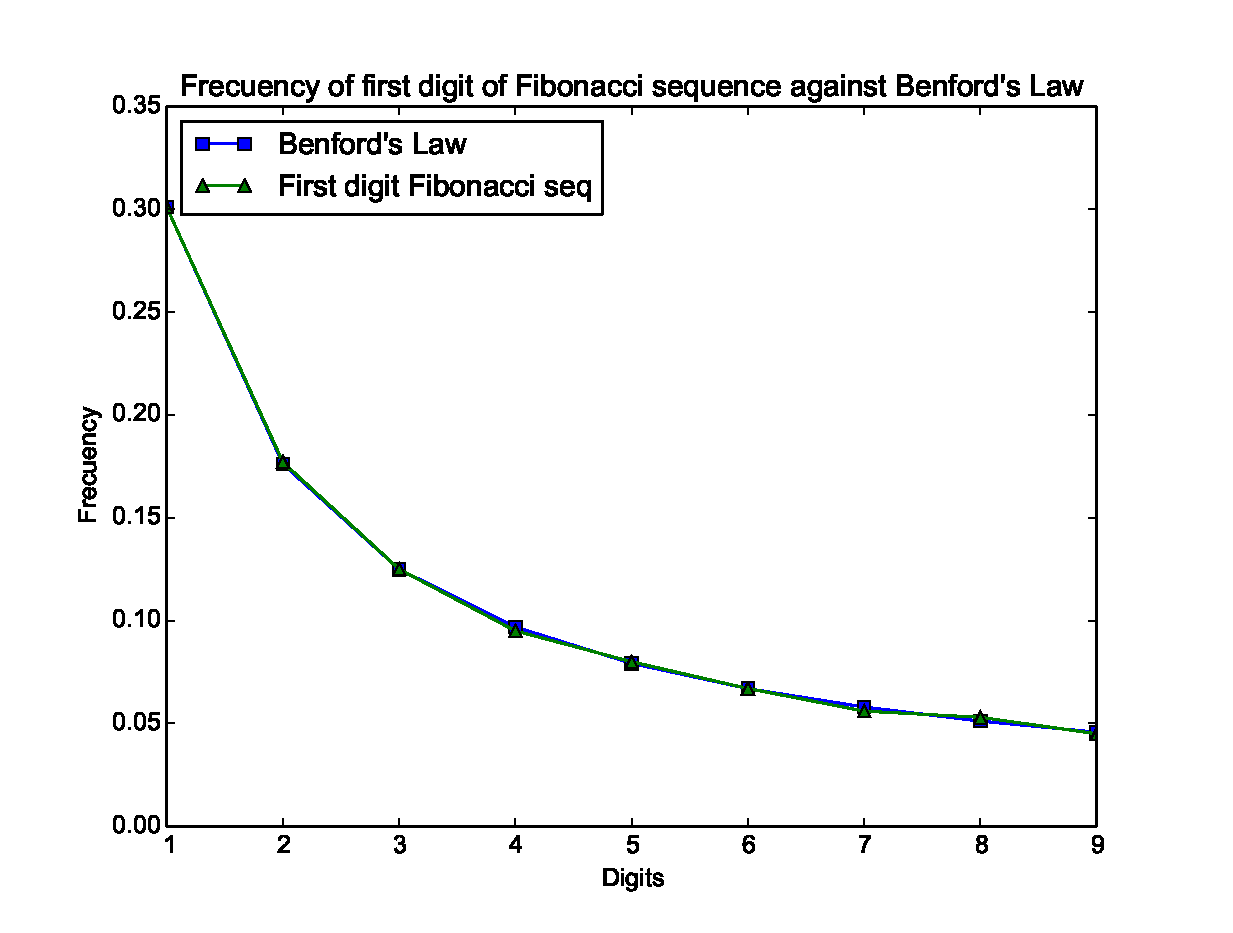
\includegraphics[scale=0.5]{imagenes/2-benford/benford_ex1}
\caption{Fibonacci Sequence against Benford's Law}
\end{figure}


\subsubsection{Mexico's Municipalities Population}
From the Mexico's National Institute of Geography and Statistics, INEGI, data from the 2010 census can be obtained. That year, 2351 Municipalities where censused and information is freely available at the institute web \href{http://www3.inegi.org.mx/sistemas/iter/entidad_indicador.aspx?ev=5}{page}.

As with the first example, the most significant digit of the population of each municipality was taken, and the frequency of repetition of each digit between 1 and 9 was compared with the prediction made by Benford's Law.

\begin{figure}[h!]
\centering
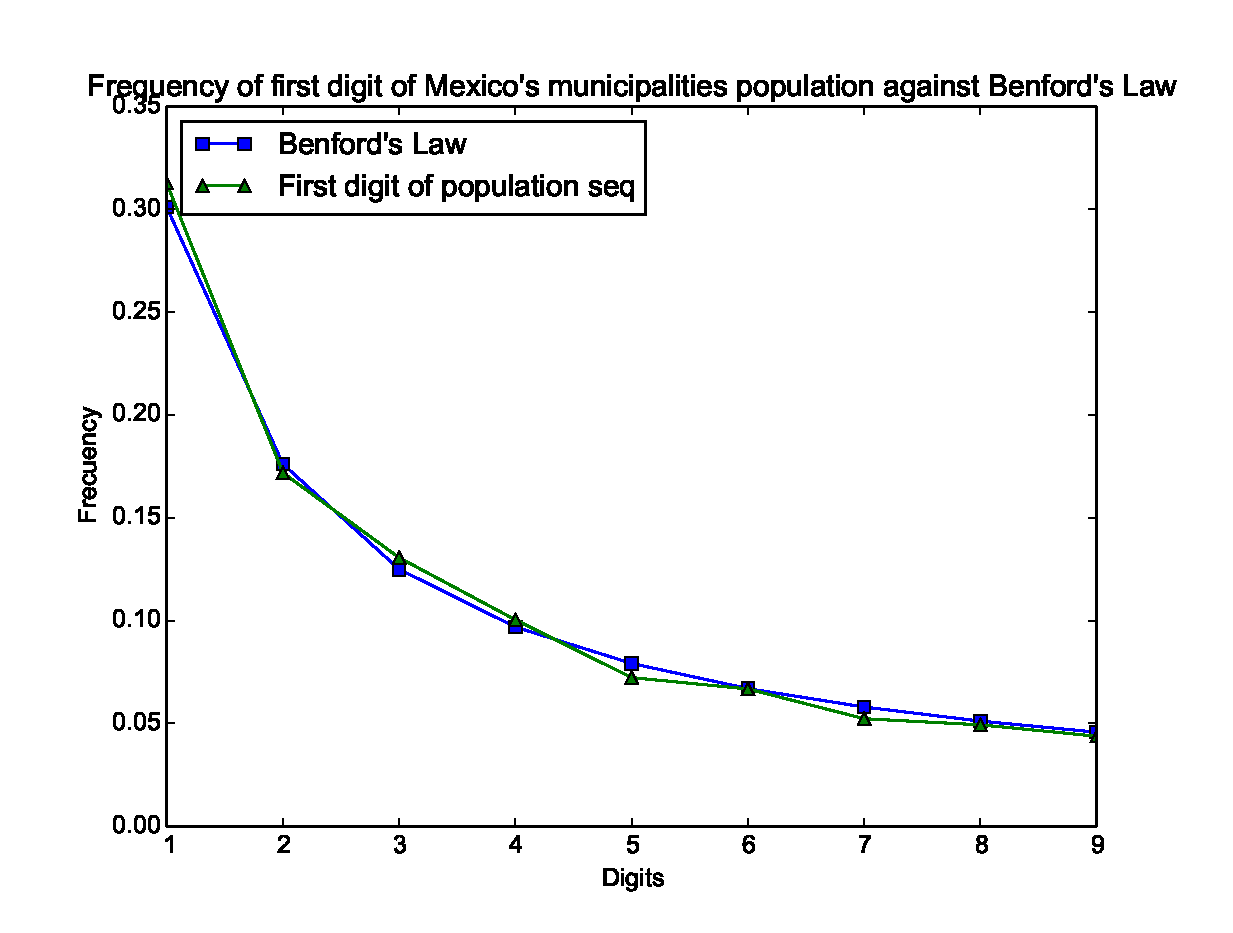
\includegraphics[scale=0.5]{imagenes/2-benford/benford_ex2}
\caption{Fibonacci Sequence against Benford's Law}
\end{figure}


\newpage
\subsection{Autonomous Circuits}
An Autonomous Circuit is a circuit that produces a time-varying output without having a time-varying input\cite{Kennedy95}. More formally:\\

An electronic circuit is described by a system of ordinary differential equations of the form:
\begin{equation*}
\dot{\mathbf{X}}(t)=\mathbf{F}(\mathbf{X}(t),t)
\end{equation*}
Where $\mathbf{X}(t)=(X_1(t),X_2(t),...,X_n(t))^T \in \mathbb{R}$ is called the \emph{state vector} and $\mathbf{F}$ is called the \emph{vector field}. $\dot{\mathbf{X}(t)}$ denotes the derivative of $\mathbf{X}(t)$ with respect to time.

If the vector field $\mathbf{F}$ depends explicitly on $t$, then the system is said to be \emph{non-autonomous}. If the vector field depends only on the state and is \emph{independent} of time $t$, then the system is said to be \emph{autonomous} and may be written in the simpler form:\\
\begin{equation}\dot{\mathbf{X}}=\mathbf{F}(\mathbf{X})\end{equation}


The time evolution of the state of an autonomous electronic circuit from an initial point $\dot{\mathbf{X}}$ at $t$=0 is given by\\

\begin{align*}\phi(\mathbf{X_0})=\mathbf{X_0}+\int_o^t\mathbf{F}(\mathbf{X}(\tau))d\tau &, t \in \mathbb{R}_+\end{align*}

The solution $\phi(\mathbf{X_0})$ is called a \emph{trajectory} through $\mathbf{X_0}$, and the set ${\phi(\mathbf{X_0}),t \in \mathbb{R}_+}$ is an \emph{orbit} of the system (1.1). The collection of maps ${\phi_t}$ that describe the evolution of the entire state space with time is called the \emph{flow}.

An autonomous electronic circuit is an example of a \emph{deterministic dynamical system}.

\subsection{Defining Chaos}
\emph{Chaos} is aperiodic long-term behavior in a determinisic system that exhibits sensitive dependence on initial conditions \cite{Strogatz14}
\begin{itemize}
\item \emph{Aperiodic long-term behavior} means that there are trajectories which do not settle down to fixed points, periodic orbits, or quasiperiodic orbits as $t$->$\inf$.
\item \emph{Deterministic} means that the system has no random or noisy inputs or parameters. The irregular behavior arises from the system's nonlinearity, rather than from noisi driving forces.
\item \emph{Sensitive dependence on initial conditions} means that nearby trajectories separate exponentially fast, i.e., that the system has a positive Lyapunov Exponent
\end{itemize}

\subsubsection{Lyapunov Exponent}
The lyapunov exponent of a dynamical system is a quantity that characterizes the rate of separation of infinitesimally close trayectories\cite{Parlitz92}.\\

Suppose that we let transients decay, so that a trajectory is \emph{on} the attractor. Suppose $\mathbf{\phi}(x,t)$ is a point on the attractor at time $t$, and consider a nearby point $\mathbf{\phi}(t)+\delta(t)$ where $\delta$ is a very small separation. It can be seen in the following figure, that  $\delta(t)$ grows. The two trajectories diverge with at a rate given by

$\lVert\delta(t) \rVert \ \lVert\delta_oo \rVert e^{\lambda t}$


\begin{figure}[h]
\centering
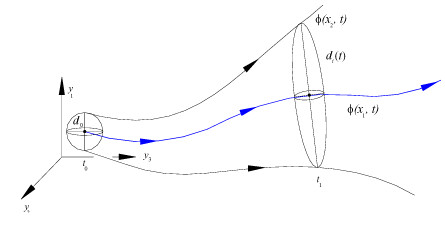
\includegraphics[scale=0.5]{imagenes/2-benford/Lyap_exp.jpg}
\caption{Neighboring trajetories separating exponentially fast with initial separation $\delta_0$ }
\end{figure}
When at least one Lyapunov exponent is positive the attractor possesses the property of sensitive dependence of initial conditions.


\subsubsection{Chua's Circuit}
\begin{itemize}\item \textbf{Chua's Oscillator}
\newline Leon Chua did research regarding Lorenz's equations\cite{Ayrom86}\cite{Kennedy95}, and deviced a chaotic electronic circuit with only one non-linear element, which is a 5-segment piecewise-linear resistor.


\begin{figure}[h]
\centering
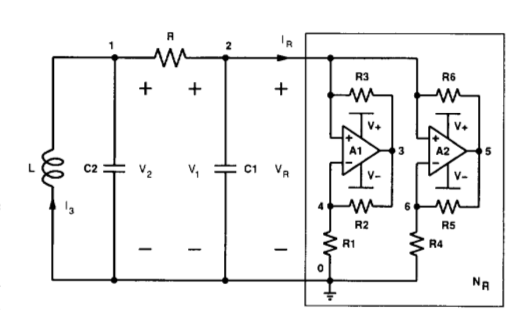
\includegraphics[scale=0.5]{imagenes/2-benford/chuas_circuit.png}
\caption{Schematic of Chua's Circuit }
\end{figure}

The dynamics of the system can be modeled by the system of three nonlinear ordinary differential equations:\\
\begin{align}
 \frac{dV_1}{dt}&=\frac{G}{C_1}(V_2-V_1)-\frac{1}{C_1}f(V_1)\\
 \frac{dV_2}{dt}&=\frac{1}{C_2}I_3-\frac{G}{C_2}(V_2-V_1)\\
 \frac{dI_3}{dt}&=-\frac{1}{L}V_2\\
\end{align}

with $G=\frac{1}{R}$ and $f(V_1)$ is given by:\\
\begin{align*}
\frac{G}{C1}V_2-\frac{G'_b}{C_1}V_1-(\frac{G_b-G_a}{C_1})E &\quad if \quad V_1< -E\\
\frac{G}{C1}V_2-\frac{G'_a}{C_1}V_1 &\quad if \quad -E\geq v1 \leq E\\
\frac{G}{C1}V_2-\frac{G'_b}{C_1}V_1-(\frac{G_a-G_b}{C_1})E &\quad if \quad V_1>E
\end{align*}
\item \textbf{Properties}
      \begin{enumerate}
       \item \textbf{Nonlinearity:} The system of equations has a nonlinear 2-terminal resistor described by a three segment piecewise-linear v-i characteristic shown in the following figure:


            \begin{figure}[h]
            \centering
            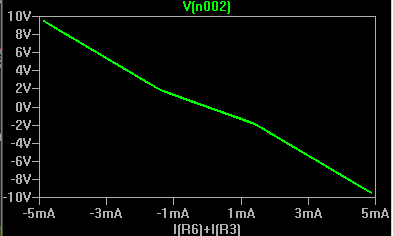
\includegraphics[scale=0.5]{imagenes/2-benford/v-i.png}
            \caption{v-i characteristic of the non-linear resistor }
            \end{figure}

      The piecewise-linear nature of the nonlinearity in Chua's Oscillator divides the state-space of the circuit into three distinct affine regions ($V_1<E$), ($\|V_1\|<E$) and ($V_1>E$)
      \item \textbf{Symmetry:}The piecewise-linear function is symmetric with respect to the origin, there exists three equilibrium points, at 0, $P_-$ and $P_+$. In the following figure, a double scroll Chua's attractor is shown. Since three equilibrium points are involved, this attractor is symmetric with respect to the origin\\

            \begin{figure}[h]
            \centering
            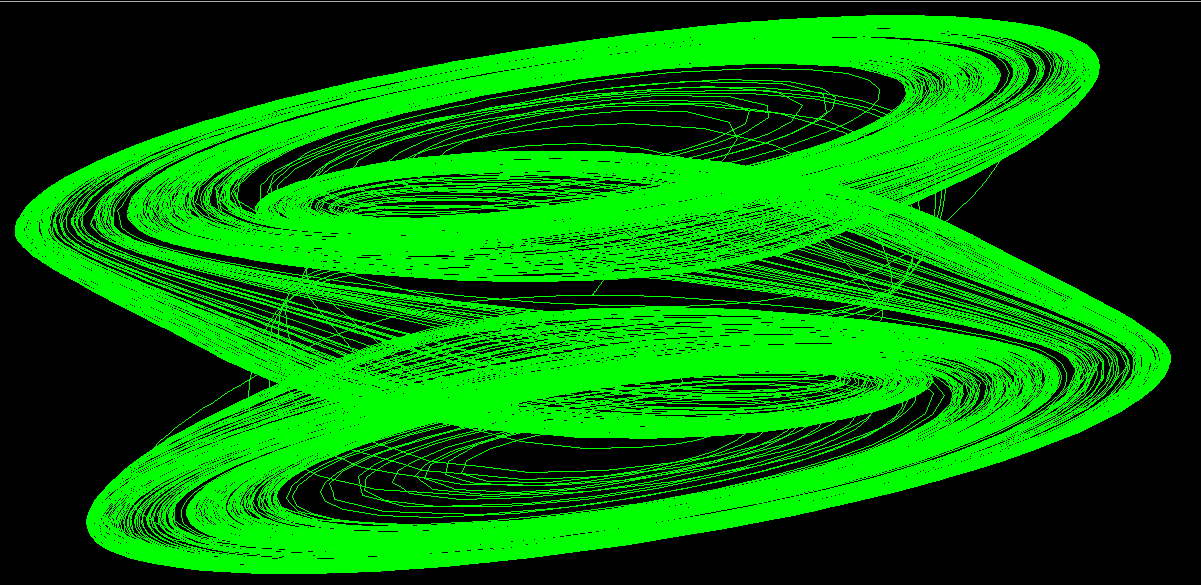
\includegraphics[scale=0.2]{imagenes/2-benford/chua_circuit.png}
            \caption{v-i characteristic of the non-linear resistor }
            \end{figure}
      \item \textbf{Dissipativity}
      \end{enumerate}
\end{itemize}


\newpage
\subsubsection{Takougang Circuit}
\begin{itemize}
\item \textbf{Three-dimensional autonomous system by Takougang et. al.}
    A three-dimensional autonomous system is presented by Sifei Takougang Kingni\cite{Takougang13}. The system exhibits chaotic bursting oscillations.\\
    The three-dimensional system is described as follows:\\
    \begin{align}
    \frac{dx}{dt}=-x+y\\
    \frac{dy}{dt}=xz-cy\\
    \frac{dz}{dt}=b-x^2-dz
    \end{align}

    where $b,c,d \in \mathbb{R}$
\item \textbf{Properties}
     \begin{itemize}
     \item \textbf{non-linearity:} Non-linearity given by the term $x^2$ and $xz$
     \item \textbf{symmetry:} Under the transformation defined by $(x,y,z) \rightarrow (-x,-y,-z)$, the system has a natural symmetry

     Next, we show that the system is symmetric.\\
     \textbf{Definition:}Let $f$ be a smooth function $f:\mathbb{R}^n \rightarrow \mathbb{R}^n$ and let\\
 \begin{align*}\mathbf{\dot{x}}=f(\mathbf{x})\end{align*}\\
 be a system of ordinary differential equations. In addition, let $\gamma$ be an invertible matrix. Then $\gamma$ is a \emph{symmetry} of the ordinary differential equation if \\
     \begin{align*}f(\gamma \mathbf{x})=\gamma f(\mathbf{x})\end{align*}

     Now, given the equation of the three-dimensional autonomous system, under the transformation $(x,y,z) \rightarrow (-x,-y,-z)$, to verify that this transformation is a symmetry of the autonomous equation, we observe that the symmetry is associated with the matrix $\gamma$ defined as\\
  \begin{align}
\gamma =
\begin{bmatrix}
-1 & 0 &0 \\
0 & -1 & 0\\
0 & 0 & 1
\end{bmatrix}
\end{align}

let \\  \begin{align}
\mathbf{\dot{x}}=f(\mathbf{x}) =
\begin{bmatrix}
-x + y \\
xz-cy\\
b-x^2-dz
\end{bmatrix}
\end{align}
with $\mathbf{x}^T=(x,y,z)$

Now, we proceed to show that $\gamma f(\mathbf{x})=f(\gamma \mathbf{x})$:\\
On the left hand side:
  \begin{align*}
\gamma f(\mathbf{x})&=
\begin{bmatrix}
-1 & 0 &0 \\
0 & -1 & 0\\
0 & 0 & 1
\end{bmatrix} \begin{bmatrix}
-x+y \\
xz-cy\\
b-x^2-dz
\end{bmatrix}\\
&=\begin{bmatrix}
x-y \\
-xz+cy\\
b-x^2-dz
\end{bmatrix}\\
\end{align*}

And now, on the right hand side:\\
  \begin{align*}
   f(\gamma \mathbf{x})&= f\left (\begin{bmatrix}
-1 & 0 &0 \\
0 & -1 & 0\\
0 & 0 & 1
\end{bmatrix} \begin{bmatrix}
x \\
y\\
z
\end{bmatrix} \right)\\
&=f\left ( \begin{bmatrix}
x \\
y\\
z
\end{bmatrix}\right )
&=\begin{bmatrix}
x-y \\
-xz+cy\\
b-x^2-dz
\end{bmatrix}
  \end{align*}

 Since the left hand side is equal to the right hand side, then $\gamma$ is a symmetry of the Three-dimensional Autonomous System. In other words, all solutions are either symmetric themselves, or have a symmetric partner
\item \textbf{Dissipativity} The system with the general condition for dissipativity (or Volume contraction):\\
         \begin{align*}\nabla V &= \frac{\partial(\frac{dx}{dt})}{\partial x}+\frac{\partial(\frac{dy}{dt})}{\partial y}+\frac{\partial(\frac{dz}{dt})}{\partial z}\\
&=-(1+c+d)
 \end{align*}

 So

\begin{align*}
V'(t)=-(1+c+d)V\\
V(t)V(0)e^{-(1+c+d)}t
\end{align*}

Thus volumes in phase space shrink exponentially fast
An explanation of dissipativity is given in \cite{Strogatz14} page 320.

\item \textbf{Fixed Points} The system has two types of fixed points:\\

      \begin{align*}
      0&=-x+y   \quad &\Rightarrow x=y\\
      0&=xz-cy   \quad&\Rightarrow z=c\\
      0&=b-x^2-dz  \quad&\Rightarrow x^2+dz=b \Rightarrow x=y=\sqrt{b-dc}
      \end{align*}
When $b \leq dc$ the fixed points for $x,y=0$ and $z=\frac{d}{b}$
When $b > dc$ the fixed points are $(\pm\sqrt{b-cd},\pm\sqrt{b-cd},c)$

\item \textbf{Sensitivity to initial conditons} Starting the system with slightly different initial conditions $(0, 0.1, 0)$ and $(0, 0.09, 0)$ we can see that after some time the two trajectories quickly diverge from each other



            \begin{figure}[h]
            \centering
            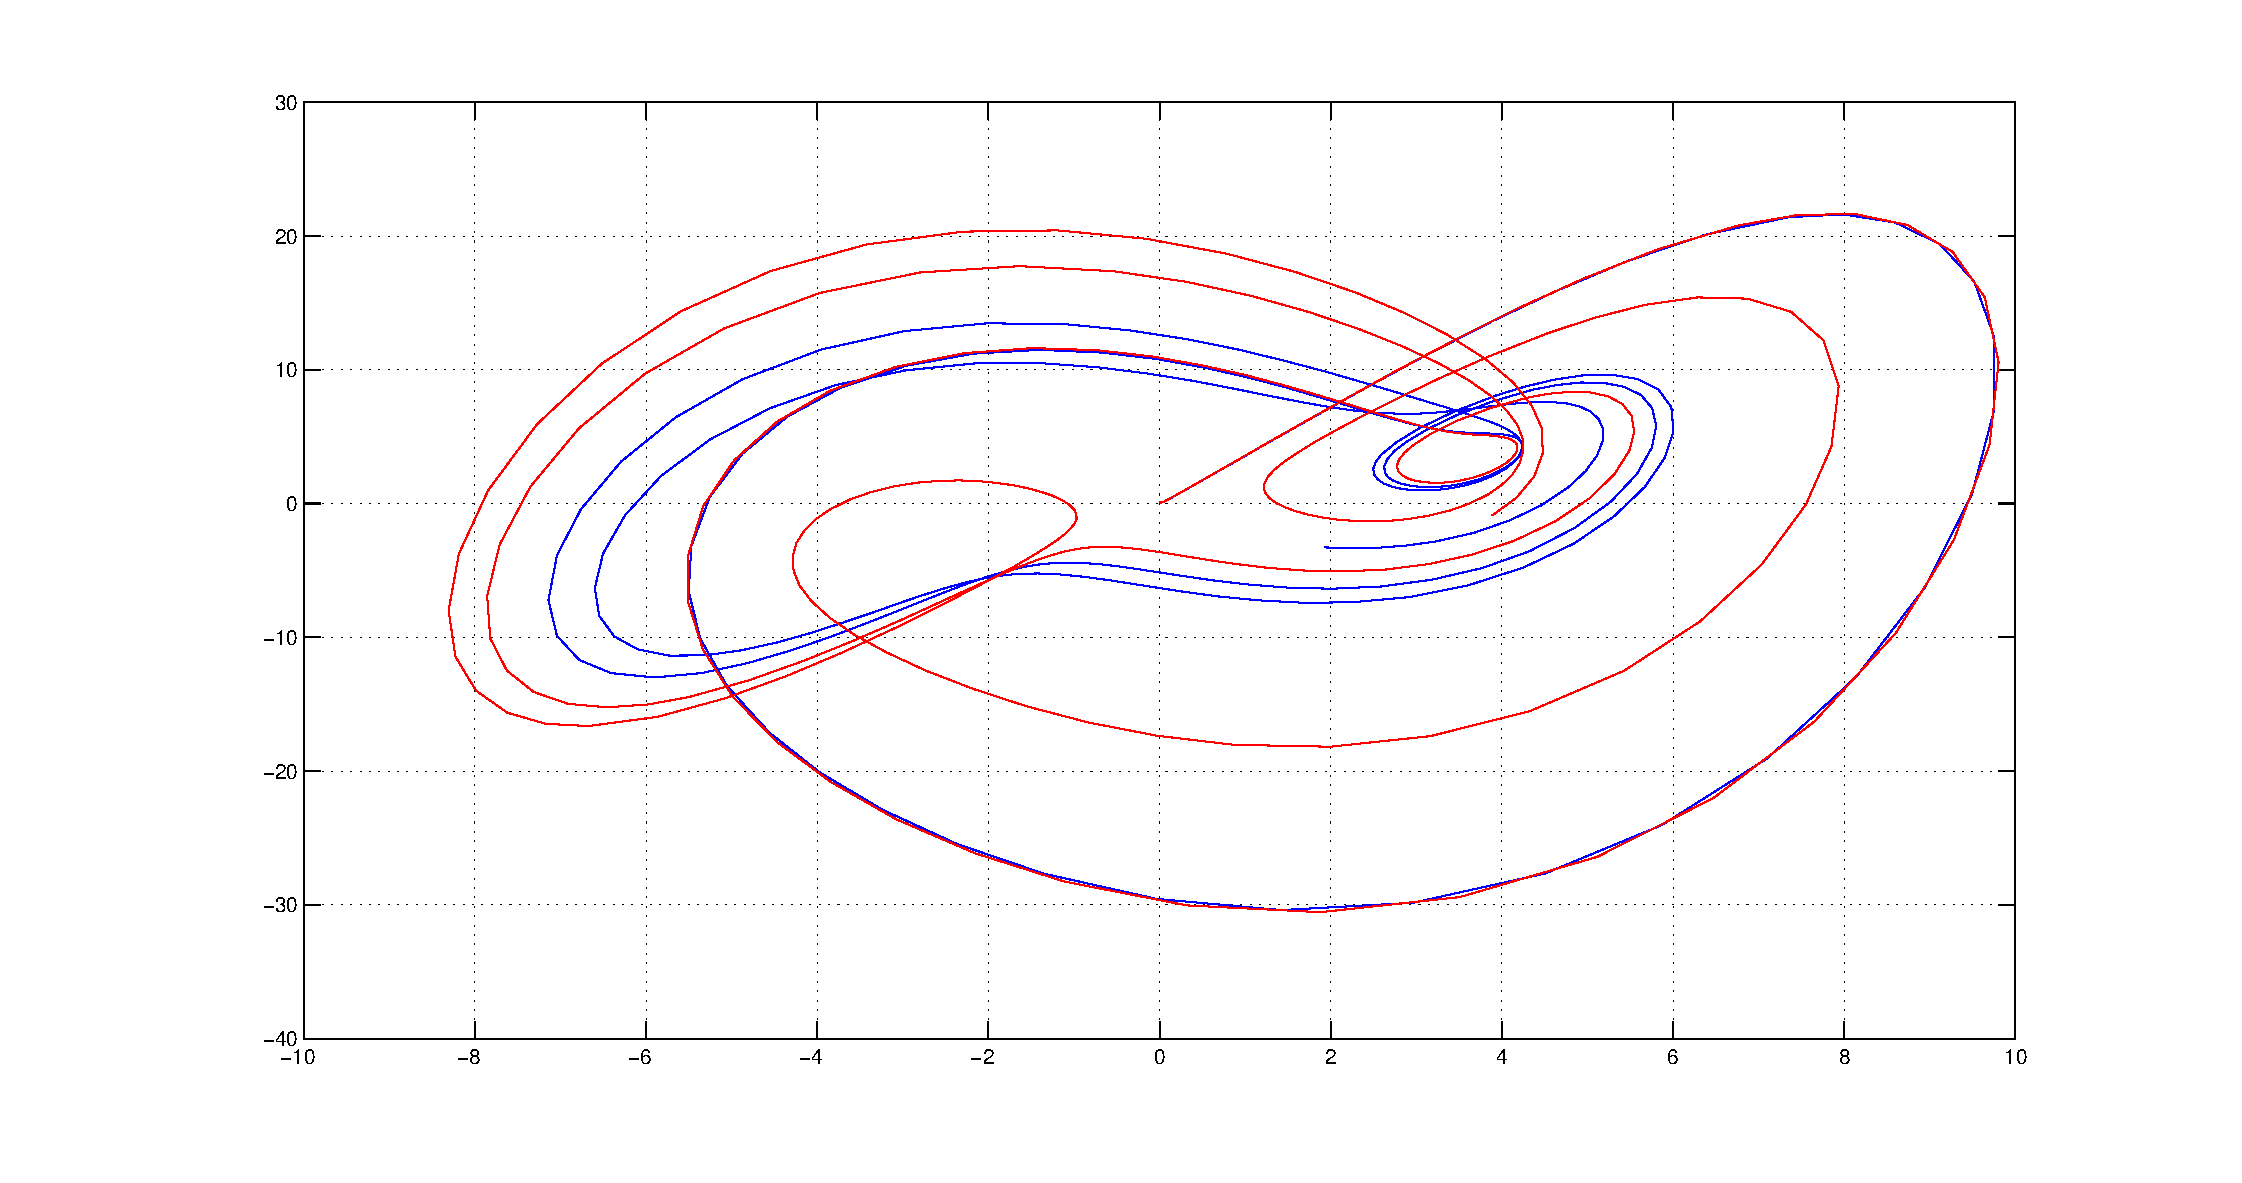
\includegraphics[scale=0.4]{imagenes/2-benford/in_cond.eps}
            \caption{Sensitivity to initial conditions in a Third Order Autonomous System}
            \end{figure}

     \end{itemize}
\end{itemize}

\cite{Takougang13} Shows that the system presents chaos of horseshoe type.


\newpage
\section{Simulations}
Simulations with Chua's System and the system proposed by \cite{Takougang13} were used to see if any of the system follows Benford's Law. On one hand we used Simulink and MATLAB in order to produce bifurcation diagrams and set up the dimensionless differential equations. On the other hand, we used a SPICE-based circuit simulator in order to get the systems in terms of electrical components.

\subsubsection{Chua's Circuit}
 \begin{itemize}
   \item \textbf{Physical Realization}
 The system describing chua's System
\begin{align*}
\frac{G}{C1}V_2-\frac{G'_b}{C_1}V_1-(\frac{G_b-G_a}{C_1})E &\quad if \quad V_1< -E\\
\frac{G}{C1}V_2-\frac{G'_a}{C_1}V_1 &\quad if \quad -E\geq v1 \leq E\\
\frac{G}{C1}V_2-\frac{G'_b}{C_1}V_1-(\frac{G_a-G_b}{C_1})E &\quad if \quad V_1>E
\end{align*}
is given by the following schematic
            \begin{figure}[H]
            \centering
            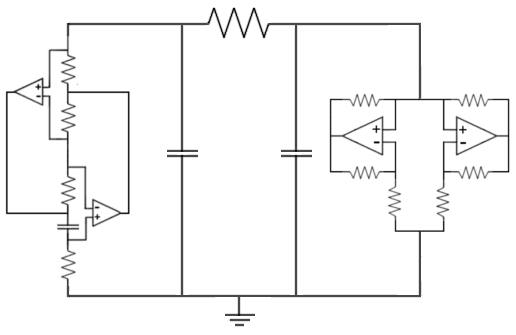
\includegraphics[scale=0.4]{imagenes/2-benford/chuas_circuit_realized.jpg}
            \caption{OP-Amp Based realization of Chua's Circuit}
            \end{figure}

With the Capacitors
C1=10nF
C2=100nF
and a 8mH Inductor given by the gyrator circuit.

   \item \textbf{Numerical Simulations}
   Using a spice based simulation software and MATLAB, several resistor values where tested, we constructed the bifurcation diagram and plotted for some R values
\begin{figure}
         \centering
            \begin{subfigure}[b]{0.4\textwidth}
            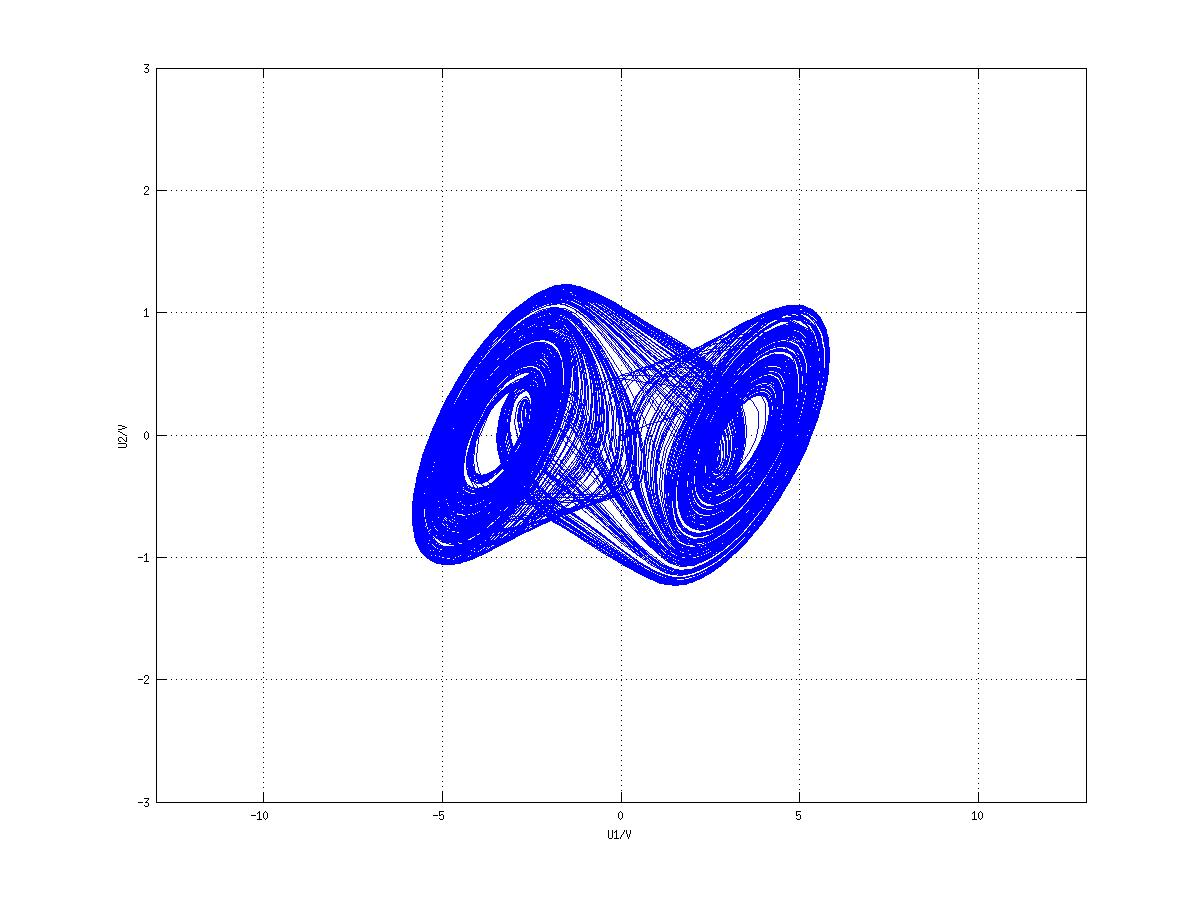
\includegraphics[width=\textwidth]{imagenes/2-benford/1785.jpg}
            \caption{V1-V2 plane for R=1785}
            \end{subfigure}
            \begin{subfigure}[b]{0.4\textwidth}
            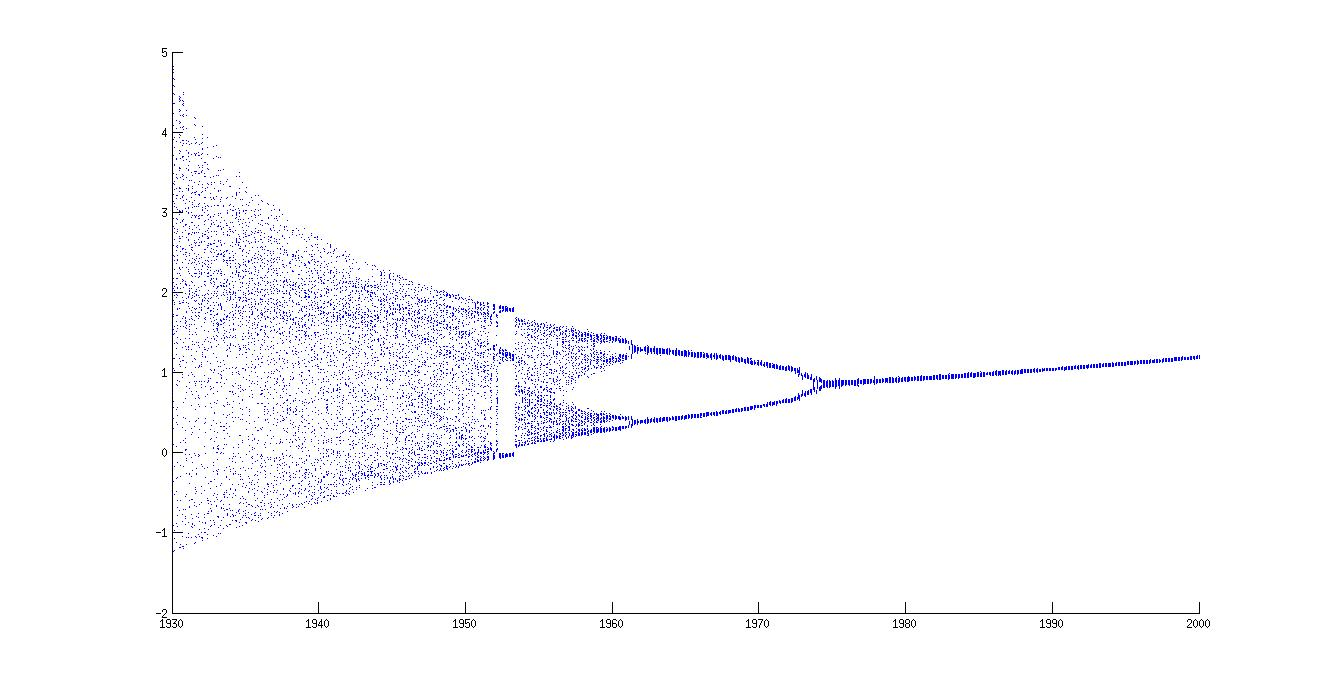
\includegraphics[width=\textwidth]{imagenes/2-benford/bifurcation_chua.jpg}
            \caption{Bifurcation Diagram for Chua's Circuit}
            \end{subfigure}
\end{figure}
   \item \textbf{Benford Analysis}
          The first digit distribution was determined from the voltage measured at the terminals of C1, using a resistance value of 1860$\Omega$, at that value, Chua's Circuit presented Chaotic Behaviour. The first digits (without leading zeroes) of the voltage values at discrete points were analyzed. We compared the first digit distribution of the dataset with the distribution given by Benford's Law using the Mean Absolute Deviation (MAD) proposed by \cite{Nigrini97}. We got a MAD value of 0.22, with a maximum of 0.15 in order to be conformant with Benford's Law.
            \begin{figure}[H]
            \centering
            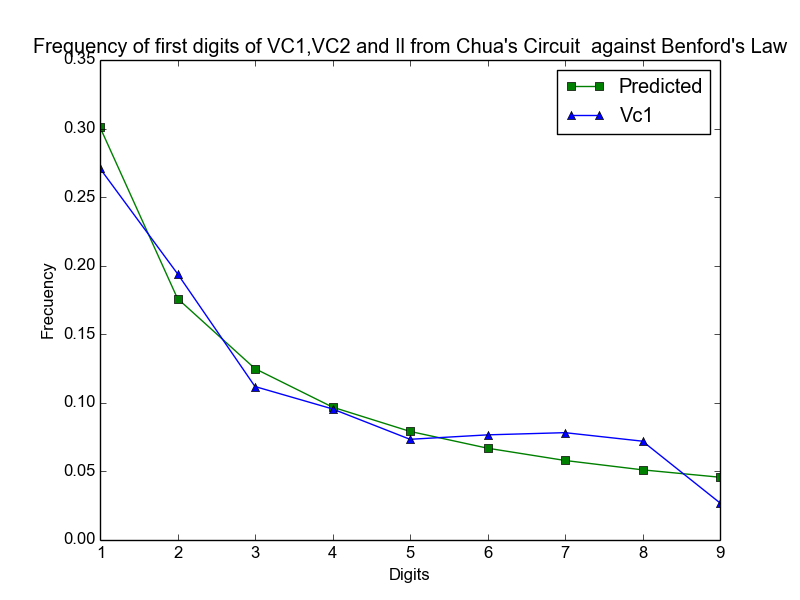
\includegraphics[scale=0.5]{imagenes/2-benford/chua_benford.png}
            \caption{OP-Amp Based realization of Chua's Circuit}
            \end{figure}
 \end{itemize}

\newpage
\subsubsection{Three-Dimensional Autonomous Circuit}
  \begin{itemize}
   \item \textbf{Physical Realization}
    The electronic circuit built to realise the system is shown in figure 2.4:
            \begin{figure}[H]
            \centering
            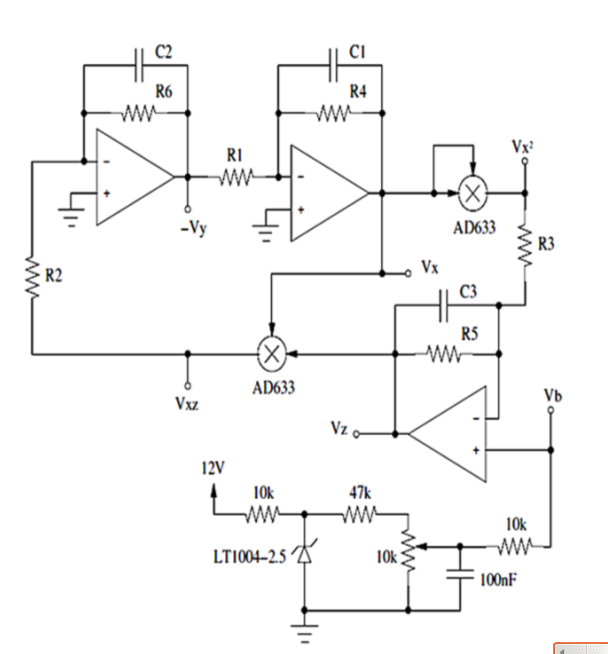
\includegraphics[scale=0.3]{imagenes/2-benford/Circuit2_schem.png}
            \caption{Circuit Schematic}
            \end{figure}
Voltages $V_x$,$V_y$ and $V_z$ are the output voltages of the operational amplifiers representing $x$,$y$ and $z$, $k_m=10V$ is the fixed constant of the AD633  multipliers, so the outputs of the multipiers are $V_{xz}=V_xV_z/k_m$ and $V_{x^2}=V_xV_x/k_m$.

            Substitution of resistor values into Eqs. (1.5),(1.6),(1.7) yields:

\begin{align}
\frac{dV_x}{dt}=\frac{1}{R_1C_1} \left ( V_y -V_x\frac{R_1}{R_4} \right )\\
\frac{dV_y}{dt}=\frac{1}{R_2C_2} \left ( \frac{V_xV_z}{k_m}-\frac{R_2}{R_6}V_y \right )\\
\frac{dV_z}{dt}=\frac{1}{R_3C_3} \left ( V_b\left ( 1+\frac{R_3}{R_5} \right )  -\frac{V_x^2}{k_m} - \frac{R_3}{R_5}V_z\right )
\end{align}

The values for resistors and capacitor used where: $R_1=0.5\text{ K}\Omega, \quad R_2=10\text{ K}\Omega, \quad R_3=10\text{ K}\Omega, \quad R_4=5\text{ K}\Omega, \quad R_5=1.15\textbf{\text{ M}}\Omega, \quad R_3=1\text{ M}\Omega, \quad C_1=100\text{ nF}, \quad C_2=100\text{ nF}, \quad C_3=10\text{ nF}, \quad V_b=10\text{ K}\Omega$
   \item \textbf{Numerical Simulations}
We used SIMULINK in order to model the system and MATLAB to create the bifurcation diagram.
            \begin{figure}[H]
            \centering
            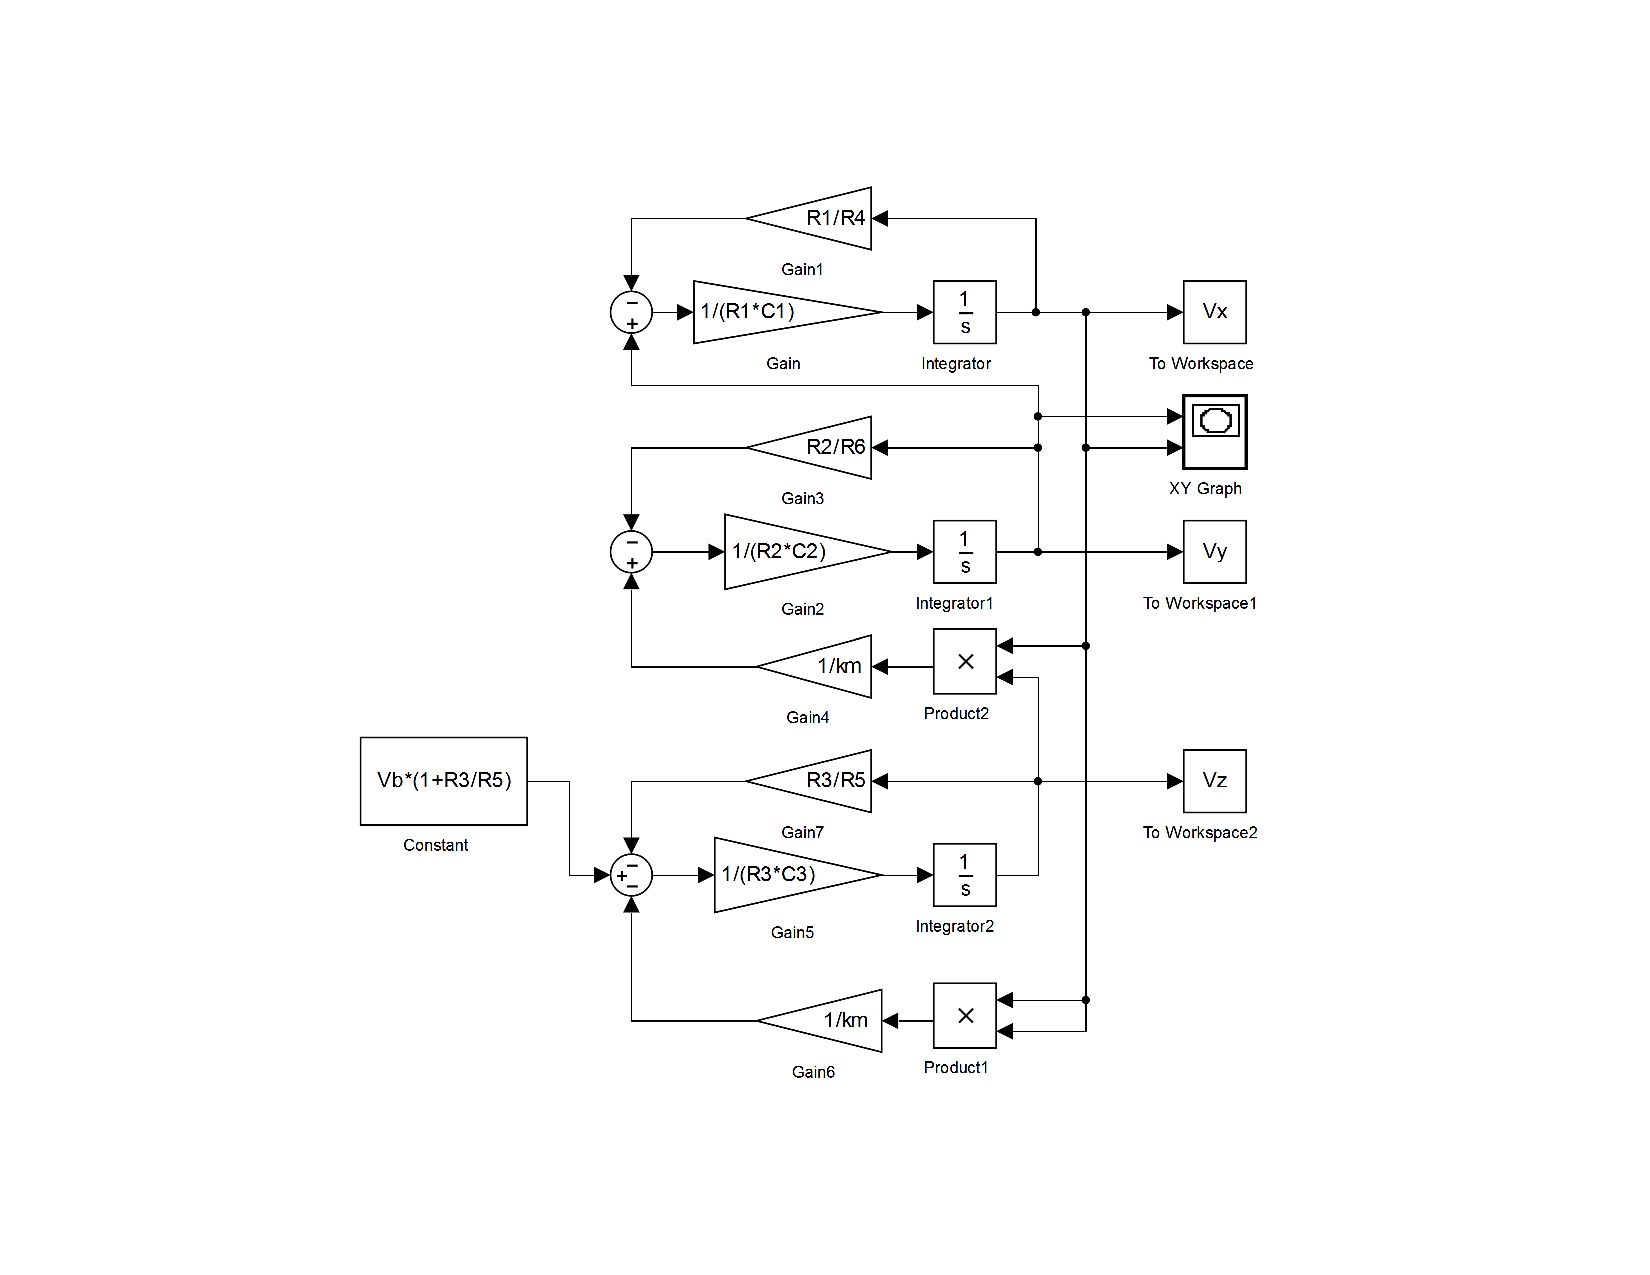
\includegraphics[scale=0.4]{imagenes/2-benford/shilkinovsimu.png}
            \caption{Simulink simulation}
            \end{figure}
The response of the syste with the parameters indicated above is given by figure 2.5:

\begin{figure}[H]
         \centering
            \begin{subfigure}[b]{0.4\textwidth}
            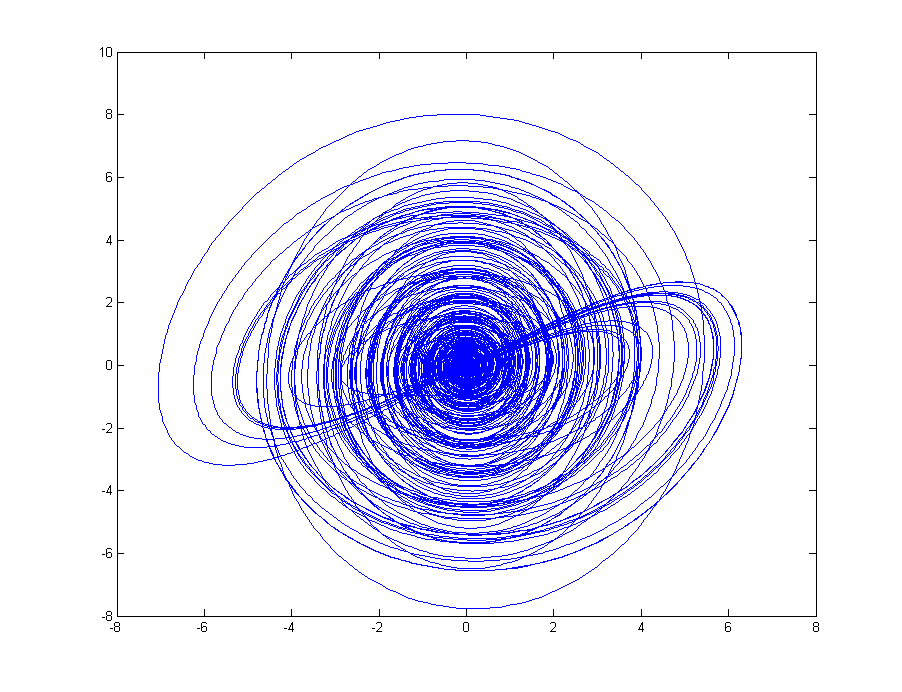
\includegraphics[width=\textwidth]{imagenes/2-benford/shilkino_resp.png}
            \caption{V1-V2 $V_x$ vs $V_y$ plot}
            \end{subfigure}
            \begin{subfigure}[b]{0.8\textwidth}
            \includegraphics[width=\textwidth]{imagenes/2-benford/bif_shil_osc_z.eps}
            \caption{Bifurcation Diagram varying b}
            \end{subfigure}
\end{figure}

Bifurcation diagram for the z value

   \item \textbf{Correspondence with Benford's Law} The same methodology used in Chua's Circuit was used with this circuit, taking measurements from $V_y$ and using the MAD test to verify conformity with the First Digit Distribution

            \begin{figure}[H]
            \centering
            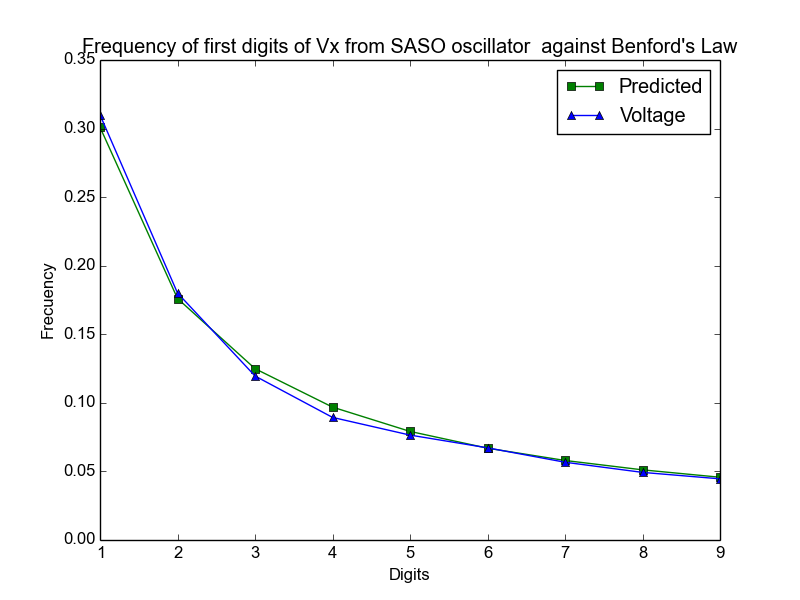
\includegraphics[scale=0.4]{imagenes/2-benford/Sh_vy.png}
            \caption{$V_x$ against Benford's Law}
            \end{figure}
For different values of d, we did a table with the respective first digit frequencies (10000 samples)  and MAD test.

\begin{center}
  \begin{tabular}{ c | c | c | c | c | c | c }
    \hline
    Leading digit  & Benford Distribution & d=1/23 &d=0.03 &d=0.01& d=0.001 &d=0.00001 \\ \hline
1&		0,3010&	0,3296&	0,3132&	0,3166&	0,2792&	0,3108\\ \hline
2&		0,1760&	0,1787&	0,1800&	0,1801&	0,1707&	0,1781\\ \hline
3&		0,1249&	0,1111&	0,1142&	0,1196&	0,1209&	0,1230\\ \hline
4&		0,0969&	0,0856&	0,0910&	0,0894&	0,0904&	0,0941\\ \hline
5&		0,0791&	0,0727&	0,0791&	0,0765&	0,0754&	0,0731\\ \hline
6&		0,0669&	0,0604&	0,0647&	0,0672&	0,0670&	0,0691\\ \hline
7&		0,0579&	0,0581&	0,0602&	0,0567&	0,0596&	0,0565\\ \hline
8&		0,0511&	0,0565&	0,0511&	0,0493&	0,0515&	0,0496\\ \hline
9&		0,0457&	0,0473&	0,0465&	0,0446&	0,0415&	0,0457\\ \hline
MAD&  & 0,0085&	0,0042&	0,0044&	0,0053&	0,0031\\ \hline

  \end{tabular}
\end{center}
We noticed strong agreement given by Nigrini\cite{Nigrini97}, next, we built the circuits and do tests measuring voltages.

 \end{itemize}


\newpage
\section{Experimental Results}
\subsubsection{Chua's Circuit}
 \begin{itemize}
  \item \textbf{Methodology}
We constructed the circuit using 4 TL082 I.C.'s and commercial resistors with the values used during simulation, Trimmer resistors to be able to move the resistor values of R.

            \begin{figure}[h]
            \centering
            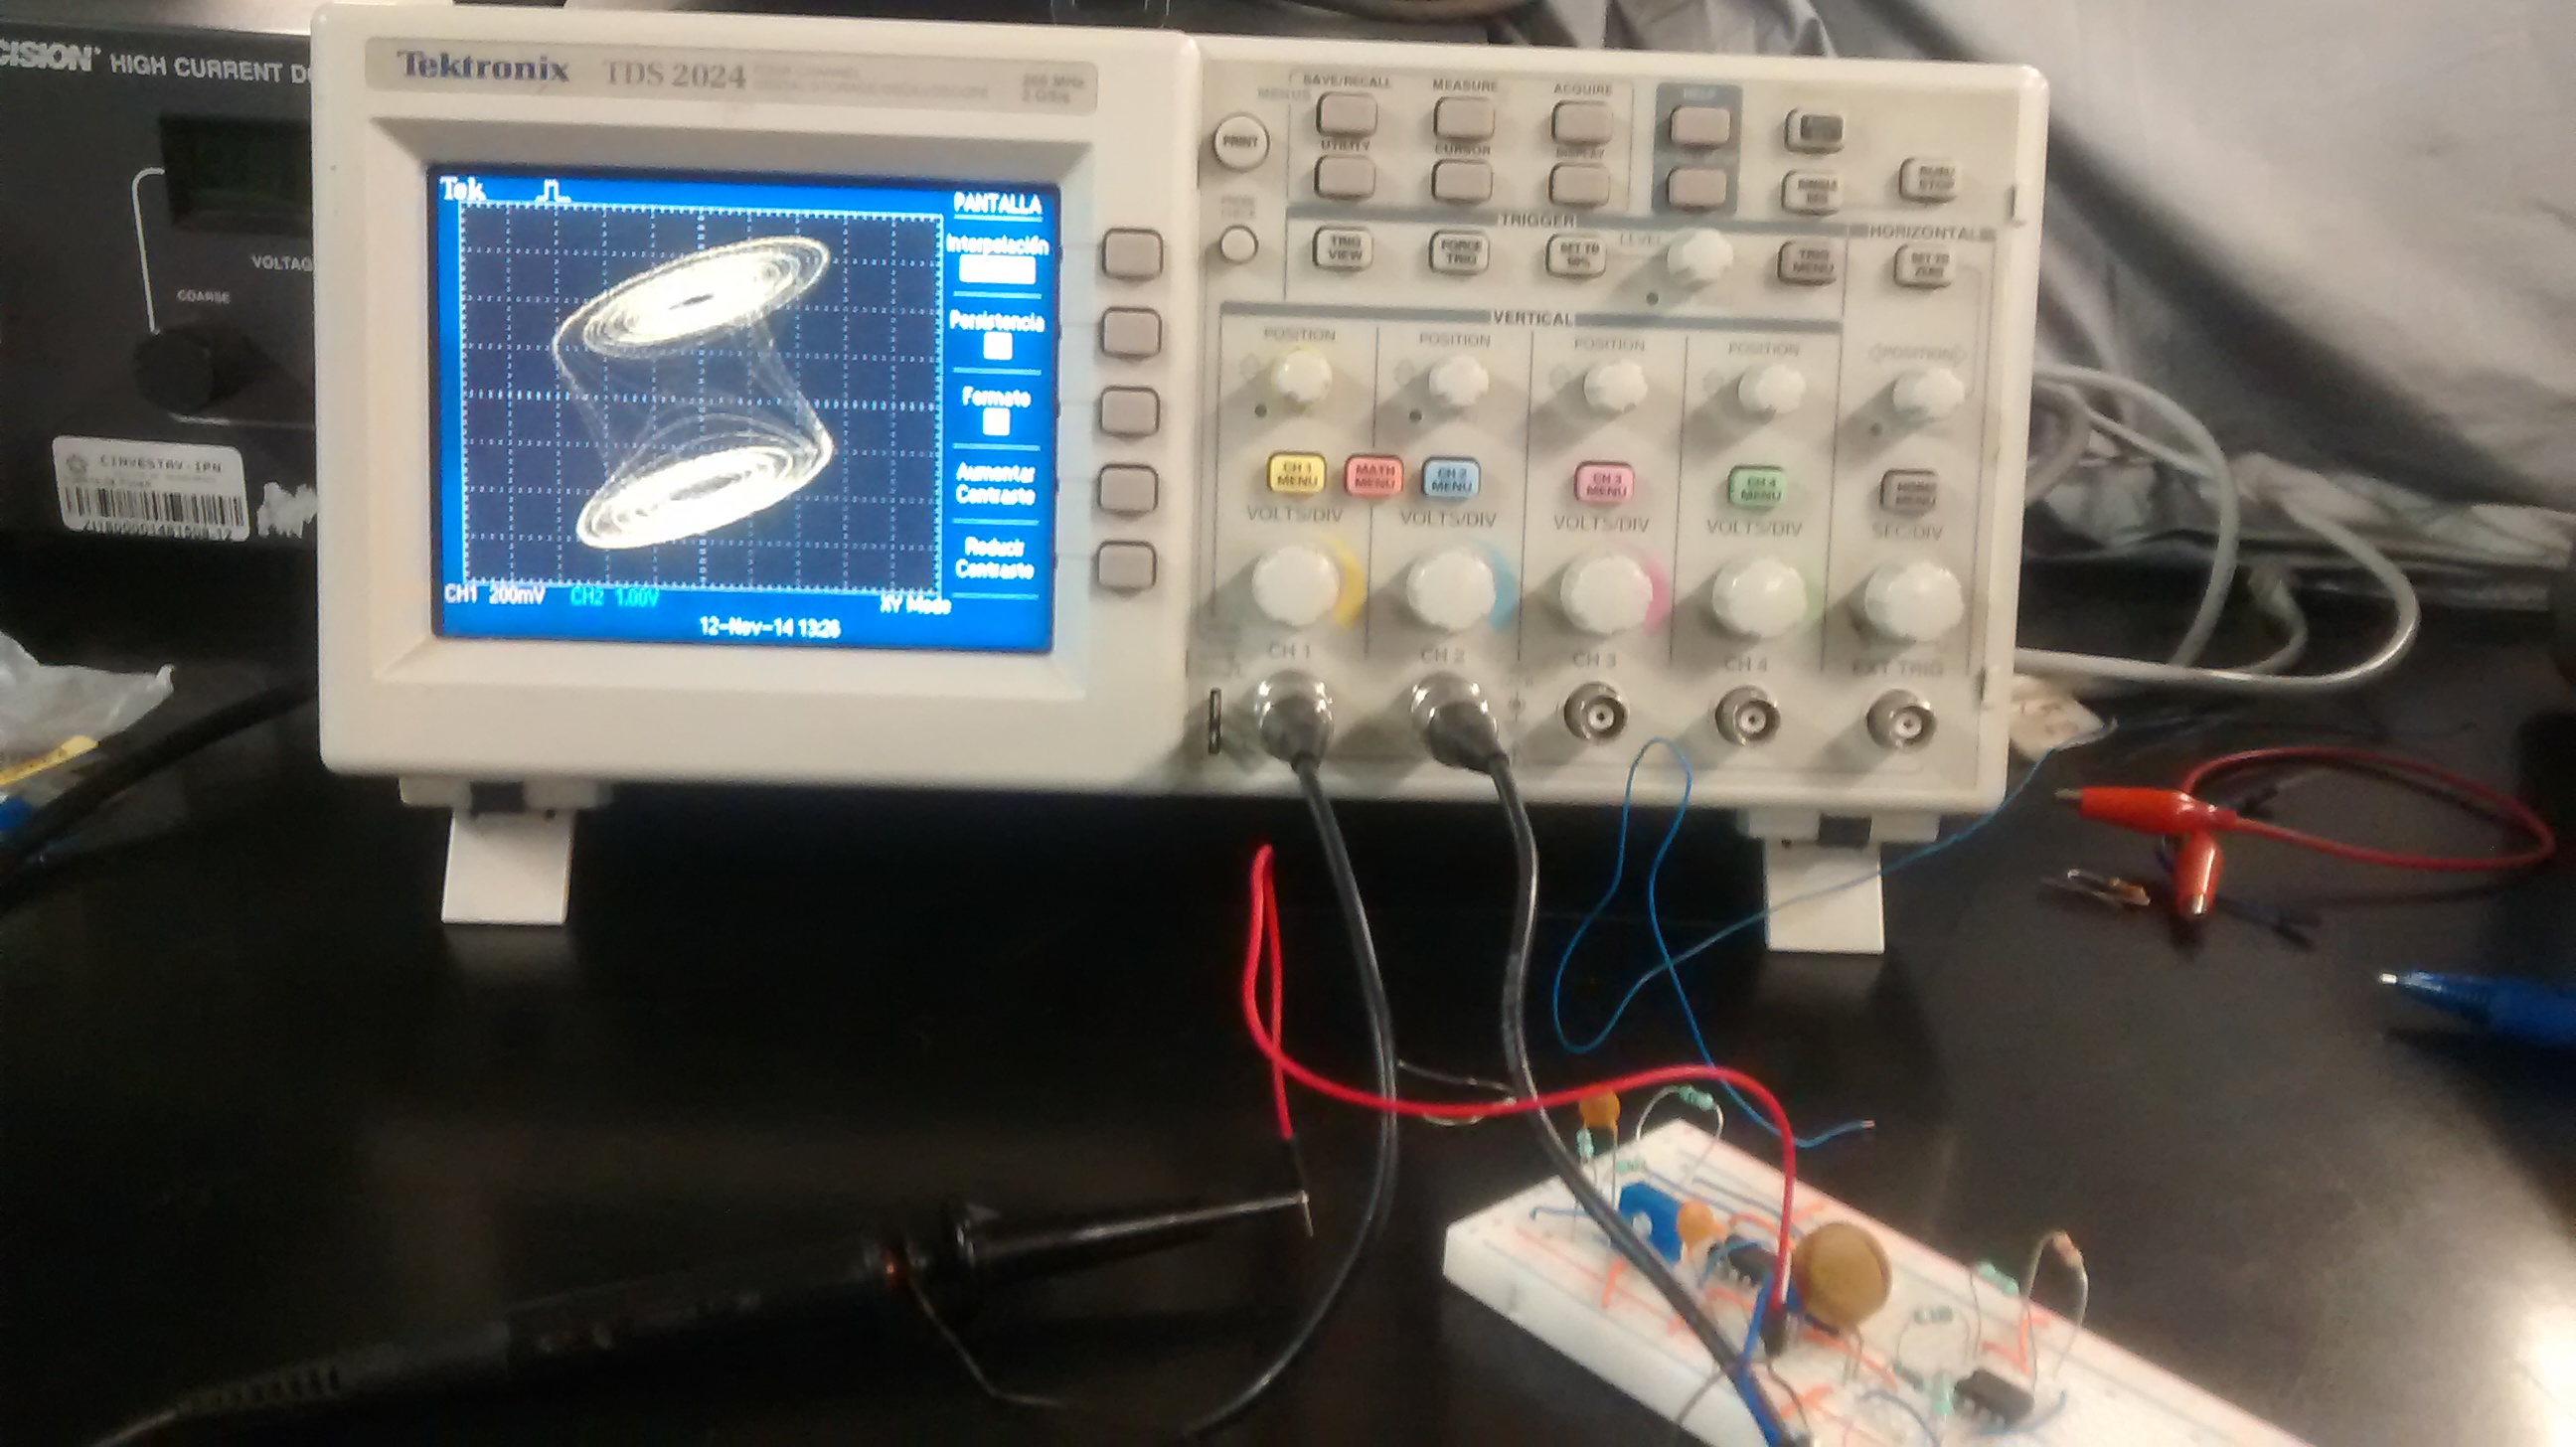
\includegraphics[scale=0.1]{imagenes/2-benford/chua_breadboard.jpg}
            \caption{Chua's System Breadboard}
            \end{figure}
We used two oscilloscope probes to measure the voltage from the two capacitors, and did our measurements with  a Tektronix DS201 Oscilloscope with a direct method sampling.

 The first digit distribution was determined from the voltage measured at the terminals of C1,varying R from 1700$\Omega$ to 1900$\Omega$in $25\Omega$ intervals, values in which Chua's Circuit presented chaotic behaviour. The first digits (without leading zeroes) of the voltage values at discrete points were analyzed, the oscilloscoped allowed us to take 2000 samples from a 250 $\mu$s period. We compared the first digit distribution of the dataset with the distribution given by Benford's Law using the Mean Absolute Deviation (MAD) proposed by \cite{Nigrini97}.



  \item \textbf{Results}
We put a table with the MAD results at each value of R:
\begin{center}
  \begin{tabular}{ c | c | c }
R & VC1 & VC2\\
1700 & 0.0265740826252 &0.0941252615083\\ \hline
1725 &  0.0308583854254& 0.0894910362566\\ \hline
1750 & 0.0225012003889 & 0.0937811348396\\ \hline
1775 &  0.0213932963068 & 0.0894482136018\\ \hline
1800 &  0.0515553953624& 0.0817178075546\\ \hline
1825 & 0.0620516456615 &0.0757908400412\\ \hline
1850& 0.0801858066881 &0.0616474503737\\ \hline
1875 & 0.0864648516751& 0.0566898036332\\ \hline
1900 &0.0848654579991 &0.0477795566486\\ \hline


  \end{tabular}
\end{center}

The closest value we got was with R=1775 measuring VC1
            \begin{figure}[h]
            \centering
            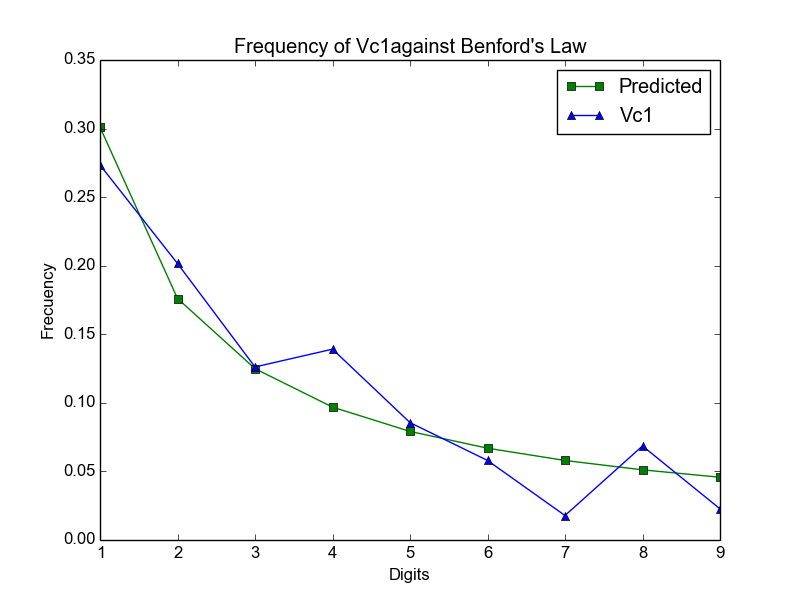
\includegraphics[scale=0.4]{imagenes/2-benford/benford_chua1775.png}
            \caption{Benford's Law against VC1}
            \end{figure}
  \item \textbf{Remarks}

We noticed that between for R between 1730 and 1775, there is a more clear First Digit Distribution according to Benford's Law, however, the measurements did not comply with MAD's Criteria which expects at most 0.015 in order to be compliant with Benford's Law. We also took a measurement with R=2000$\Omega$, value at which the system behaves as a quasi-periodic oscillator. we noticed that the first digit distribution is more uniform.

\begin{figure}
         \centering
            \begin{subfigure}[b]{0.4\textwidth}
            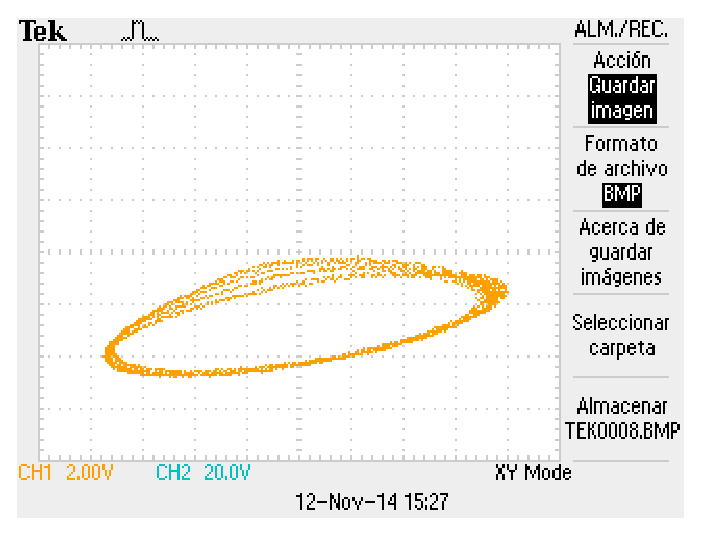
\includegraphics[width=\textwidth]{imagenes/2-benford/chua_2000.eps}
            \caption{V1-V2 $V_x$ vs $V_y$ plot}
            \end{subfigure}
            \begin{subfigure}[b]{0.8\textwidth}
            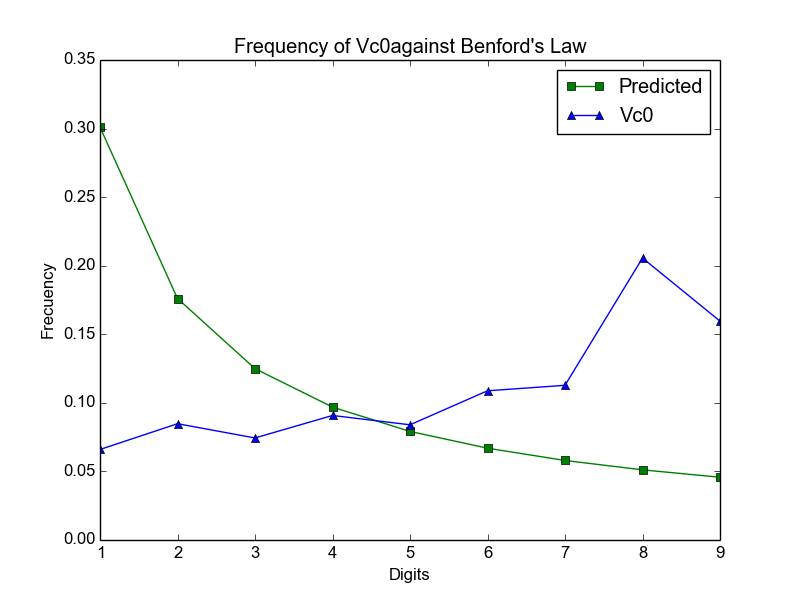
\includegraphics[width=\textwidth]{imagenes/2-benford/benford_chua20.png}
            \caption{Bifurcation Diagram varying b}
            \end{subfigure}
\end{figure}

 \end{itemize}
\subsubsection{Takougang Circuit}
 \begin{itemize}
  \item \textbf{Methodology}The circuit was connected using a standard breadboard, according to the diagram, all passive components had a nominal value equal to the ones proposed in the schematic, with a tolerance of 5\%. A regulated voltage source, set to $\pm$ 12 V was utilized to feed the active components which were the same as stated in the schematic. A third output of the regulated voltage source served to provide a stable input for the circuit ($V_b$). Next, a digital oscilloscope was used in order to obtain the data provided by the circuit.

A 1 GHz band-width oscilloscope (Agilent DSO6104A) was used next, and it was configured in order to reduce random noise. The sampler uses an averaging algorithm which delivers data with less noise, and reduces the vertical resolution (as low as 0.7 mV), with the data obtained from that oscilloscope the analysis was more reliable and results confirmed what was expected from the simulations, although only 1000 samples in an interval of 10 ms were fetched.
  \item \textbf{Results}
The first digit distribution of the voltages was taken and following the same methodology as with Chua's System, we swept through $V_b$ and took the MAD value from each distribution
\begin{center}
  \begin{tabular}{ c | c | c }
    \hline
$V_b$  & $V_x$&$V_y$\\ \hline
82mV & 0.0775279989288 & 0.0607280417648 \\ \hline
92mV & 0.0789296997697 &  0.0620760330126 \\ \hline
102mv & 0.0779822062934 & 0.0620098514762  \\ \hline
112mv & 0.0722551588234 & 0.0586329019652  \\ \hline
117mv & 0.0731369417692 & 0.0565637073089  \\ \hline
122mv & 0.0761361923841 & 0.0607646781498  \\ \hline
127mv & 0.0702382876578 & 0.0581541345311  \\ \hline
132mv & 0.0726371865346 & 0.0568562424256  \\ \hline
137mv & 0.0723923763659 & 0.0588608733569  \\ \hline
142mv & 0.0689722218274 & 0.0566979795649  \\ \hline
147mv & 0.0649140903028 & 0.0492049220995  \\ \hline
152mv & 0.0689575397758 & 0.0540809650999  \\ \hline
157mv &0.071269709088 & 0.0556102788266   \\ \hline
167mv &0.0713877270204 & 0.0546276659144  \\ \hline
187mv & 0.0642837364043 & 0.0499581746439  \\ \hline
197mv &0.0619961498144 & 0.0491763886427  \\ \hline
217mv & 0.0644054740322 & 0.0521147934116  \\ \hline
237mv & 0.0574813303354 & 0.0515391121266  \\ \hline
257mv & 0.0552768884655 & 0.0514296383228  \\ \hline
277mv & 0.0464325092508 & 0.0450451557158  \\ \hline
112mv (H-Res) &0.0126362748635 & 0.0149581584175  \\ \hline
132mv  (H-Res)& 0.0114562387312 & 0.0056682935093  \\ \hline
152mv  (H-Res)& 0.0106402668795 & 0.0143777130129  \\ \hline
172mv  (H-Res)& 0.0077090293797 & 0.0118696485616  \\ \hline
192mv  (H-Res)& 0.00801241025011 & 0.0120739312228  \\ \hline

  \end{tabular}
  \end{center}

We notice we have the best agreement with Benford's Law with $V_b=132mV$ Which gives a MAD value of 0.0056

            \begin{figure}[h]
            \centering
            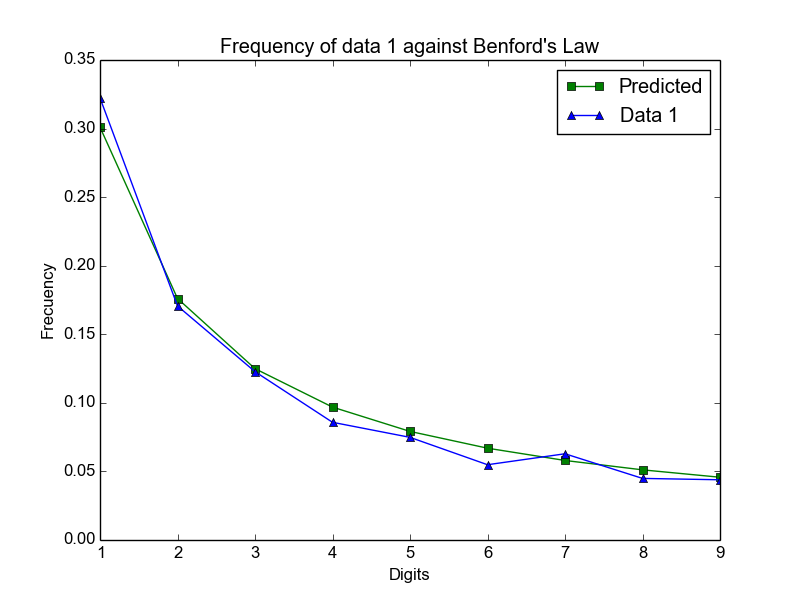
\includegraphics[scale=0.4]{imagenes/2-benford/benford_shilnikov_1.png}
            \caption{Benford's Law against digit distribution of $V_y$}
            \end{figure}

  \item \textbf{Remarks}

Simulations from Simulink gave a better accordance with $V_b=132mV$, however measuring without High-resolution sampling we did not obtain proper distributions, until we activated that sampling method, we got a distribution according to Benford's Law
 \end{itemize}


\section{Conclusion}
In the work done by Tolle \cite{Tolle00} some dynamical systems were proposed and theye checked if the first digit distribution followed Benford's Law. We took 2 autonomous circuits which displayed chaotic behaivour and verified if they were conformant according with the criterion given by Nigrini et. al. \cite{Nigrini97}. According to our experimental results, the system which best followed the distribution whas the Third Order Autonomous System proposed by Takougang et.al \cite{Takougang13}.

Verifyng the results from \cite{Takougang13}, we notice that this circuit has a Shilnikov heteroclinic orbit, which implies by the Shilnikov Criterion that the system has horseshoe chaos. This type of chaos produces time signals called chaotic bursting oscillations (see Fig. 4.1)
\begin{figure}[h]
            \centering
            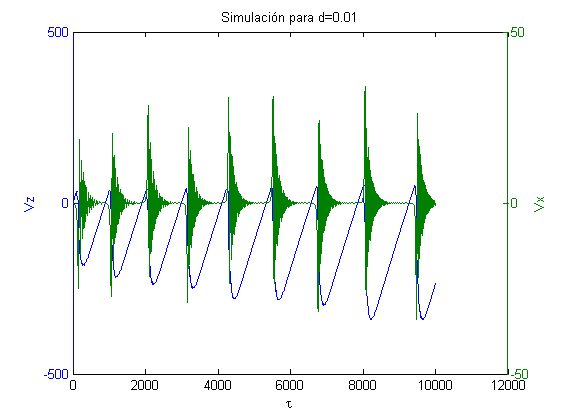
\includegraphics[scale=0.6]{imagenes/2-benford/bursting_oscilatons.png}
            \caption{$V_y$ response as a function of time}
            \end{figure}


This type of oscillations are found in biological phenomena, such as $Ca^2+$ oscillations in non-excitable cells \cite{Perc03}, pancreatic $\beta$ cells \cite{Sherman88} and in neurons\cite{Ermentrout09} and heart oscillatons, also, the work by Kreuzer et. al. \cite{Kreuzer14} indicates that brain electrical activity follows Benford's Law, so it would be interesting to see if Benford's Law could be an indicative if Real life phenomena is modelled correctly by the system if both follow Benford's Law (as it was first indicated by \cite{Tolle00}) and also to try to verify if other systems that present this kind of oscillations also follow Benford's Law.

%----------------------------------------------------------------------------------------
%  BIBLIOGRAPHY
\begin{thebibliography}{1}

\bibitem{Benford38}
  Benford Frank,
  \emph{The law of anomalous numbers}.
  Proc. Amer. Philos. Soc. 78,
  (1938),
  551-572.

\bibitem{Nigrini97}
  Nigrini Mark J., Mittermaier Linda J.
  \emph{The use of Benford's Law as an Aid in Analytical Procedures}
  Auditing: A Journal of Practice \& Theory,
  (1997),
  52-67

\bibitem{Kreuzer14}
  Matthias Kreuzer, Denis Jordan, PhD, Bernd Antkowiak, Berthold Drexler, Eberhard F. Kochs, and Gerhard Schneider
  \emph{Brain Electrical Activity Obeys Benford's Law}
  Neuroscience in Anesthesiology and Perioperative Medicine,
  (2014),
  183-191
\bibitem{Strogatz14}
 Steven H. Strogatz
  \emph{Nonlinear Dynamics and Chaos, With Applications to Physics, Biology, Chemistry and Engineering, Second Edition}
  Westview Press,
  (2014),
  309-191
\bibitem{Parlitz92}
  U. Parlitz
  \emph{Lyapunov's Exponent from Chua's Circuit}
  Journal of Circuits, Systems, and Computers,Vol. 3, No.2
  (1992),
  507-523
\bibitem{Kennedy95}
  Michale Peter Kennedy
  \emph{Experimental Chaos from Autonomous Electronic Circuits}
  Phil. Trans. R. Soc. Lond. A,
  (1995),
  507-523

\bibitem{Ayrom86}
Ayrom F.,
 \emph{Chaos in Chua's Circuit},
 IEE Proceedings, Vol. 133, No. 6 307-312
 , 1986,
 307-312


\bibitem{Takougang13}
Sifeu Takougang Kingni, Lars Keuninckx, Paul Woafo,  Guy Van der Sande, Jan Danckaert
\emph{Dissipative chaos, Shilnikov chaos and bursting oscillations
in a three-dimensional autonomous system: theory
and electronic implementation}
Nonlinear Dynamics,
2013

\bibitem{Torres07} Torres J. et al.,
 \emph{How do numbers begin? (The first digit law)},
  Eur. J. Phys., Vol. 28,
   2007,
   17-25

\bibitem{Tolle00}
Charles R. Tolle, Joanne L. Budzien, and Randall A. LaViolette
\emph{Do dynamical systems follow Benford’s law?}
Chaos: An Interdisciplinary Journal of Nonlinear Science 10,
 331,
2000
\bibitem{Perc03}
Perc, M., Marhl, M.
\emph{ Different types of bursting calcium
oscillations in non-excitable cells},
Chaos Solitons Fractals 18,
 759–773
2003
\bibitem{Sherman88}
Sherman, A., Rinzel, J., Keizer, J.
\emph{ Emergence of organized bursting in clusters of pancreatic $\beta$-cells by channel sharing},
Biophys. J. 54, 411–425,
1988
\bibitem{Ermentrout09}
\emph{Mathematical Foundations of Neuroscience}
Interdiscplinary Applied Mathematics 35,
103-126,
2009
\end{thebibliography}

% \end{document}


    \chapter{Dinámica Agro-Socio-Ambiental en la conservación de la biodiversidad en México mediante la regulación de la calidad de la Matriz Agrícola}
    
% \renewcommand{\tablename}{Tabla}
% \renewcommand{\listtablename}{Índice de Tablas}
% \renewcommand{\listfigurename}{Índice de Figuras}
% \begin{titlepage}
% \begin{center}
% 
\includegraphics[width=0.15\textwidth]{imagenes/cinvestav}~\\[1cm]
%
% \textsc{\LARGE CINVESTAV-IPN}\\[1.5cm]
%
% \textsc{\Large Proyecto Final Modelado y Simulación}\\[0.5cm]
%
% % Title
% \HRule \\[0.4cm]
% { \huge \bfseries Dinámica Agro-Socio-Ambiental en la conservación de la biodiversidad en México mediante la regulación de la calidad de la Matriz Agrícola\\[0.4cm] }
%
% \HRule \\[1.5cm]
%
% % Author and supervisor
% \noindent
% \begin{minipage}{0.4\textwidth}
% \begin{flushleft} \large
% \emph{Autores:}\\
% \begin{itemize}
% \item[$\bullet$] Alan Osorio Orduña
% \item[$\bullet$] Sergio Naude Citalán
% \end{itemize}
% \end{flushleft}
% \end{minipage}%
% \begin{minipage}{0.4\textwidth}
% \begin{flushright} \large
% \emph{Profesor:} \\
% D. en C. Juan Carlos Martínez García
% \end{flushright}
% \end{minipage}
% \vfill
% % Bottom of the page
% %{\large \today}
% \end{center}
% \end{titlepage}
% %\newcommand{\HRule}{\rule{\linewidth}{0.15cm}}

%\pagenumbering{Roman} % para comenzar la numeración de paginas en números romanos
\section*{Resumen}
Hoy en día las reservas naturales están siendo afectadas por la actividad humana. La producción agrícola no planificada adecuadamente, genera destrucción del hábitat alterando los ecosistemas, de tal forma que en ocasiones resulta en un daño irreversible.    \\

Disminuir el impacto ambiental provocado por las zonas de cultivo cercanas a reservas naturales sin interrumpir la producción agrícola, es una de las prioridades en diferentes partes del mundo.\\

En base a estudios que sean realizados en los últimos años se piensa que la matriz agrícola es de vital importancia. Es útil ver de manera gráfica y numérica los efectos que el hombre causa en la naturaleza. Razón por la cual se recopilo información de diferentes fuentes, todas relacionadas con el cultivo de café en Chiapas. Los datos recopilados fueron almacenados en una base de datos, para después ser utilizados para el modelo matemático realizado con cadenas markovianas. A partir de los resultados obtenidos en el modelo se describe la proyección a futuro de la calidad de la matriz. Los parámetros considerados para determinar la calidad de la matriz fueron de distintos ámbitos, desde flora y fauna del lugar, hasta métodos de cultivo y compuestos de plaguicidas y fertilizantes. \\

Con este proyecto se pretende configurar los parámetros necesarios para cambiar el estado de la calidad de  una matriz a otro, o por el contrario mantenerlo en un tiempo determinado.\\

Se realizaron programas de software para visualizar y conocer el la calidad de la matriz agrícola de las zonas de cultivos con respecto a las especies que habitan en los alrededores en un tiempo especificado.\\

Para la creación y depuración del programa se usó un compilador orientado a agentes, el cual permitió ver la interacción de las especies animales con el medio.
% \newpage
% \tableofcontents % indice de contenidos
% %\addcontentsline{toc}{chapter}{Indice de contenidos} % si queremos que aparezca en el índice
% %\newpage
% %\thispagestyle{empty}
% %\listoffigures % indice de figuras
% %\addcontentsline{toc}{chapter}{Índice de Figuras} % para que aparezca en el indice de contenidos
% \newpage
% \thispagestyle{empty}
% %\listoftables % indice de tablas
% %\addcontentsline{toc}{chapter}{Índice de Tablas} % para que aparezca en el indice de contenidos
% %\newpage
% %\thispagestyle{empty}
% %\newpage


\section{Introducción}
El crecimiento urbano propicia cambios en los espacios circundantes, tales como la pérdida de áreas agrícolas y forestales a favor de los ambientes urbanizados, y cambios en las estructuras socioeconómicas relacionadas con el manejo y propiedad de la tierra.\\

Chiapas es un estado con un fuerte crecimiento pero que aún mantiene áreas forestales, que cuentan con esquemas de protección de sus bosques.\\

El efecto del crecimiento urbano es complejo y no unidireccional, pues representa una fuerte presión para el cambio de uso del suelo, pero también ha permitido la reactivación de actividades agrícolas de bajo impacto y la revalorización de las áreas forestales.\\

Chiapas es conocido por su alta diversidad de especies de mamíferos, sin embargo, en la entidad grandes extensiones de hábitats naturales han sido modificados a zonas agrícolas, lo cual se cree que disminuye la riqueza de especies.\\

Por ello, el presente trabajo tiene como objetivo determinar la riqueza de suelo en zonas agrícolas del estado de Chiapas, particularmente en las que se cultiva café. Se recopiló información de las especies de flora y fauna de la región en bases de datos del gobierno estatal y federal, así como en colecciones de literatura científicas nacionales e internacionales.

\section{Objetivos}

\begin{itemize}
\item[$\bullet$] Descripción de la dinámica espacio-temporal de los factores agro-socio-ambientales relacionados con los sistemas agrícolas que impactan la calidad de la matriz agroecológica. Mediante el empleo de dinámicas Markovianas para la descripción de la evolución de la matriz agro-ecológica y considerando la interacción de territorios aledaños mediante dinámicas de agentes.
\item[$\bullet$] Desarrollo de un simulador computacional capaz de analizar mediante sistemas de información geográfica y bases de datos disponibles el escenario del impacto de distintos tipos de manejo agrícola en diversos contextos socio- ambientales en la dinámica espacio-temporal de la matriz.
\end{itemize}

\section{Marco Teórico}
\subsection{Cadenas de Markov}
Se conoce como cadena de Márkov a un tipo especial de proceso estocástico discreto en el que la probabilidad de que ocurra un evento depende solamente del evento inmediatamente anterior. Si se conoce la historia del sistema hasta su instante actual, su estado presente resume toda la información relevante para describir en probabilidad su estado futuro.\\

Si el estado $X_n$ y los estados previos $X_1, \dots,X_{n-1}$ son conocidos. La probabilidad del estado futuro $X_{n+1}$. No depende de los estados anteriores $X_1,\dots,X_{n-1}$. Solamente depende del estado $X_n$.\\

Es decir,

\begin{itemize}
\item[$\bullet$] Para $n = 1, 2,\dots$ y
\item[$\bullet$] Para cualquier sucesión de estados $s_1,\dots,s_{n+1}$.
\end{itemize}

\begin{multline}
    P(X_{n+1} = s_{n+1} | X_1 = s_1, X_2 = s_2,\dots, X_n = s_n ) \\ =  P(X_{n+1} = s_{n+1} | X_n = s_n)
\end{multline}

\subsection{Matriz de transición}
En matemáticas, una matriz de Markov es una matriz utilizada para describir las transiciones en una cadena de Markov. Existen varias definiciones y tipos de matriz estocástica:

\begin{itemize}
\item Una matriz estocástica derecha es una matriz cuadrada cada una de cuyas filas está formada por números reales no negativos, sumando cada fila 1.
\item Una matriz estocástica izquierda es una matriz cuadrada cada una de cuyas columnas está formada por números reales no negativos, sumando cada columna 1.
\item Una matriz doble estocástica es una matriz cuadrada donde todos los valores son no negativos y todas las filas y columnas suman 1.
\end{itemize}

Un proceso de Markov en que el sistema posee $n$ estados posibles, dados por los números $1, 2, 3,\dots., n$. Denotemos $p_{ij}$  a la probabilidad de que el sistema pase al estado $j$ después de cualquier ensayo en donde su estado era $i$ antes del ensayo. Los números $p_{ij}$  se denominan probabilidades de transición y la matriz $n\times n$  $P = (p_{ij})$ se conoce como matriz de transición del sistema.\\

La suma $1\dots p_{i1} + p_{i2} + p_{in} = 1$. Esta suma representa la probabilidad de que el sistema pase a uno de los estados $1, 2,\dots, n$ dado que empieza en el estado $i$. Ya que el sistema ha de estar en uno de estos n estados, la suma de probabilidades debe ser igual a 1. Esto significa que los elementos en cualquier renglón de la matriz de transición deben sumar $1$.  Cada elemento $p_{ij}\geq0$.\\

De la misma manera, puede definirse un vector estocástico como un vector cuyos elementos están formados por números reales no negativos que suman 1. Así, cada fila (o columna) de una matriz estocástica es un vector de probabilidad, también llamados vectores estocásticos.

\section{Simulación}
Dentro de la simulación son usados dos programas principalmente. El primero de ellos es Matlab con una interfaz gráfica, el segundo es el programa de desarrollo de ambientes Netlogo.\\

La interfaz gráfica implementada en Matlab permite ingresar los datos de la matriz de transición. Cada elemento de la matriz y el vector de condiciones iniciales son introducidos manualmente por el usuario. Después mediante un algoritmo de iteraciones entre el vector de condiciones iniciales y la propia matriz de transición, se obtiene un vector de salida. Éste último nos indica en qué tipo de clasificación se encuentra la matriz.\\

Primero se introducen las condiciones iniciales en forma de vector fila. Dichas condiciones indican la calidad de la matriz en un inicio, en escala de 0 a 1, siendo 1 excelente calidad. En base a diversas propiedades con las que cuenta la matriz es como se le asignan las componentes al vector. En el presente trabajo los factores considerados fueron:

\begin{itemize}
\item Tipo de cultivo.
\item Fertilizantes y/o plaguicidas.
\item Calidad de sombra.
\end{itemize}

La Figura \ref{fig:1} muestra la interfaz en Matlab

\begin{center}
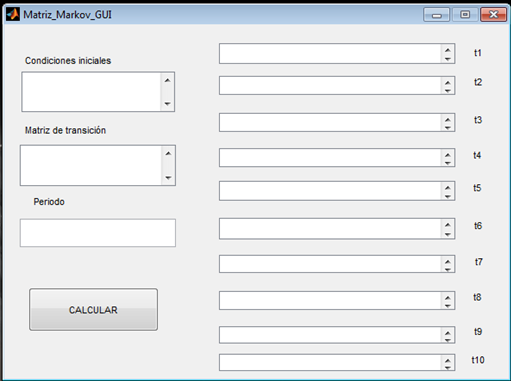
\includegraphics[scale=0.45]{imagenes/4-agricola/1.png}
\captionof{figure}{Interfaz gráfica- Matriz de Markov}
\label{fig:1}
\end{center}

La matriz de transición nos condensa las probabilidades de un estado a otro. A través de ésta matriz se puede observar el comportamiento representado por una cadena de Markov. Es decir, las propiedades de cambio entre los estados de la matriz agrícola.\\

Finalmente el periodo (en años) acota la escala de tiempo en la que se evalúa la matriz. Limitado por la información disponible, la proyección sólo se puede hacer máximo a 10 años.\\

El vector de condiciones iniciales es el siguiente:
$$\left[\begin{array}{ccc}
0{.}1&0{.}5&0{.}9
\end{array}\right]$$
La matriz de transición fijada es la siguiente:

\begin{align*}
\left[\begin{array}{ccc}
0{.}3&0{.}6&0{.}7
\end{array}\right]\\
\left[\begin{array}{ccc}
0{.}1&0{.}3&0{.}8
\end{array}\right]\\
\left[\begin{array}{ccc}
0{.}4&0{.}6&0{.}6
\end{array}\right]
\end{align*}

El programa en Netlogo muestra de manera gráfica la interacción de la matriz agrícola con especies animales. Además presenta el impacto que tienen distintos métodos de cultivo en la población de la fauna silvestre. La Figura \ref{fig:2} muestra el programa de Netlogo en ejecución.

\begin{center}
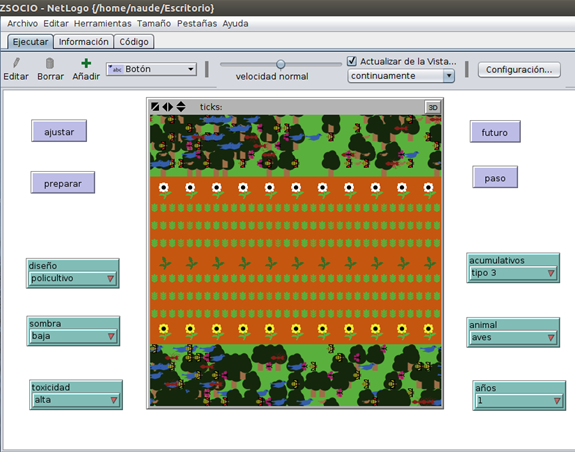
\includegraphics[scale=0.45]{imagenes/4-agricola/2.PNG}
\captionof{figure}{Interfaz en Netlogo}
\label{fig:2}
\end{center}

\section{Manual de software de simulación la calidad de la matriz agrícola de café}
\begin{enumerate}
\item Se seleccionan los parámetros de la zona agrícola.

\item Tipo de diseño, sombra, toxicidad y acumulativos.

\item Se da clic en ajustar para que muestre la zona agrícola con los parámetros deseados.

\item Se selecciona el animal con el que se pretenda visualizar como atravesara la zona agrícola con los parámetros descritos anteriormente.

\item Se presiona el botón ``preparar'' para ajustar el entorno y las variables que van estar interactuando durante el paso de la especie animal por la zona agrícola.

\item Se presiona el botón ``paso'' para que avancen cierta cantidad de espacio los animales por la zona agrícola hasta que salgan de ella.

\item Se colocan los nuevos parámetros así como la cantidad de años que a la que se quiere visualizar como se verá la matriz a tiempo futuro con los nuevos parámetros.
\end{enumerate}

\section{Conclusiones}
Se prueba la importancia de la calidad de la matriz agrícola en su entorno (en este caso es específicamente la relacionada con el cultivo de café).\\

Se visualiza de manera gráfica y numérica el impacto de la matriz con su alrededor en un tiempo finito a través de la modificación de ciertos parámetros.\\

Se encuentra la ponderación de los parámetros que puede modificar  de manera directa el hombre sobre la matriz agrícola en las zonas de cultivo de café.\\

Se logra visualizar los rangos de valores que deben tener los parámetros para reducir los daños generados por el hombre mientras realiza una actividad agrónoma,  en este caso el cultivo de café.

\bibliographystyle{ieeetr} \nocite{*}
\bibliography{xbiblioteca} %bibliografía.


    \chapter{Interacción entre el Bienestar Psicológico y el Paisaje Acústico}
        %
% \documentclass{article}
% \usepackage{amsfonts}

%%%%%%%%%%%%%%%%%%%%%%%%%%%%%%%%%%%%%%%%%%%%%%%%%%%%%%%%%%%%%%%%%%%%%%%%%%%%%%%%%%%%%%%%%%%%%%%%%%%%%%%%%%%%%%%%%%%%%%%%%%%%%%%%%%%%%%%%%%%%%%%%%%%%%%%%%%%%%%%%%%%%%%%%%%%%%%%%%%%%%%%%%%%%%%%%%%%%%%%%%%%%%%%%%%%%%%%%%%%%%%%%%%%
%TCIDATA{OutputFilter=LATEX.DLL}
%TCIDATA{Version=5.50.0.2953}
%TCIDATA{<META NAME="SaveForMode" CONTENT="1">}
%TCIDATA{BibliographyScheme=Manual}
%TCIDATA{Created=Sunday, December 14, 2014 13:08:08}
%TCIDATA{LastRevised=Sunday, December 14, 2014 18:02:07}
%TCIDATA{<META NAME="GraphicsSave" CONTENT="32">}
%TCIDATA{<META NAME="DocumentShell" CONTENT="Scientific Notebook\Blank Document">}
%TCIDATA{CSTFile=Math with theorems suppressed.cst}
%TCIDATA{PageSetup=72,72,72,72,0}
%TCIDATA{AllPages=
%F=36,\PARA{038<p type="texpara" tag="Body Text" >\hfill \thepage}
%}


% \newtheorem{theorem}{Theorem}
% \newtheorem{acknowledgement}[theorem]{Acknowledgement}
% \newtheorem{algorithm}[theorem]{Algorithm}
% \newtheorem{axiom}[theorem]{Axiom}
% \newtheorem{case}[theorem]{Case}
% \newtheorem{claim}[theorem]{Claim}
% \newtheorem{conclusion}[theorem]{Conclusion}
% \newtheorem{condition}[theorem]{Condition}
% \newtheorem{conjecture}[theorem]{Conjecture}
% \newtheorem{corollary}[theorem]{Corollary}
% \newtheorem{criterion}[theorem]{Criterion}
% \newtheorem{definition}[theorem]{Definition}
% \newtheorem{example}[theorem]{Example}
% \newtheorem{exercise}[theorem]{Exercise}
% \newtheorem{lemma}[theorem]{Lemma}
% \newtheorem{notation}[theorem]{Notation}
% \newtheorem{problem}[theorem]{Problem}
% \newtheorem{proposition}[theorem]{Proposition}
% \newtheorem{remark}[theorem]{Remark}
% \newtheorem{solution}[theorem]{Solution}
% \newtheorem{summary}[theorem]{Summary}
% \newenvironment{proof}[1][Proof]{\noindent\textbf{#1.} }{\ \rule{0.5em}{0.5em}}
% \input{tcilatex}
%
% \begin{document}


\begin{center}
CENTRO DE INVESTIGACIONES AVANZADAS DEL INSTITUTO POLIT\'{E}CNICO NACIONAL

DEPARTAMENTO DE CONTROL AUTOM\'{A}TICO

MAESTR\'{I}A EN CIENCIAS EN CONTROL AUTOM\'{A}TICO

REPORTE FINAL DE PROYECTO

\textbf{INTERACCI\'{O}N ENTRE EL BIENESTAR PSICOL\'{O}GICO Y EL PAISAJE
SONORO.}

ING. CONCEPCI\'{O}N JAZM\'{I}N SU\'{A}REZ POLO

ING. MILCOM ELIJACK PEREGRINA OCHOA

ASESOR: DR. JUAN CARLOS MART\'{I}NEZ GARC\'{I}A

\bigskip

DICIEMBRE 2014

\bigskip
\end{center}

\textbf{Indice general. }

Resumen \qquad 2

Abstract\qquad 2

1. Introducci\'{o}n\qquad 2

2. Cronograma\qquad 3

3. Estado del arte\qquad 3

3.1 Surgimiento y desarrollo del concepto de paisaje sonoro.\qquad 3

3.2 Caracter\'{\i}sticas del paisaje sonoro.\qquad 3

3.3 An\'{a}lisis del paisaje sonoro.\qquad 4

3.4 Estructura del paisaje sonoro.\qquad 5

3.5 Caracter\'{\i}sticas estructurales para el an\'{a}lisis de paisajes
sonoros.\qquad 5

4. Entrevista.\qquad 6

5. Parte Experimental.\qquad 8

5.1 Equipo de grabaci\'{o}n.\qquad 8

5.2 Grabaci\'{o}n de campo.\qquad 9

5.2.1 Paisaje sonoro natural y paisaje sonoro con elemento humano.\qquad 9

5.2.2 Paisaje sonoro urbano.\qquad 10

5.3 Edici\'{o}n y an\'{a}lisis de las grabaciones.\qquad 10

6. Dise\~{n}o de la Red Perceptr\'{o}n Multicapa con algoritmo

supervisado Backpropagation tipo gradiente.\qquad 12

6.1 Acondicionamiento de datos.\qquad 17

6.2 Entrenamiento de la red neuronal.\qquad 18

6.3 Modo de operaci\'{o}n de la aplicaci\'{o}n.\qquad 23

Conclusiones.\qquad 24

Referencias.\qquad 24

Bibliograf\'{\i}a consultada.\qquad 24

\textbf{\'{I}ndice de figuras y tablas}

Figura 1. Grabadora Tascam DR40\qquad 8

Figura 2. Aud\'{\i}fonos Sennheiser hd 205\qquad 8

Figura 3. Grabadora Tascam DR40 montada en tr\'{\i}pode y con
antiviento\qquad 9

Figura 4. Espectrograma antes y despu\'{e}s de correcciones\qquad 11

Figura 5. An\'{a}lisis de espectro en frecuencia paisaje natural, natural
con\qquad 12

elemento humano y urbano respectivamente\qquad 12

Figura 6. Datos del espectrograma.\qquad 12

Figura 7. Representaci\'{o}n de una Neurona\qquad 14

Figura 8. Funci\'{o}n sigmoidea\qquad 15

Figura 9. Espectro analizado por Audacity\qquad 18

Figura 10. Organizaci\'{o}n de los datos en hojas de c\'{a}lculo\qquad 18

Figura 11. Gr\'{a}fica en Matlab de los datos de entrenamiento\qquad 19

Figura 12. Patrones de entrenamiento\qquad 19

Figura 13. Hipermatriz de capas de la red neuronal\qquad 13

Figura 14. Matriz de Bias de la red neuronal\qquad 20

Figura 15. Resultado para 500 \'{e}pocas\qquad 21

Figura 16. Resultado para 600 \'{e}pocas\qquad 21

Figura 17. Resultado para 800 \'{e}pocas\qquad 22

Figura 18. Aplicaci\'{o}n standalone\qquad 23

Tabla 1. Cronograma de actividades.\qquad 3

Tabla 2. Rangos de sonido de la OMS\qquad 22

\textbf{Resumen }

En el presente Proyecto, se realizar\'{o}n grabaciones de campo en tres
entornos sonoros distintos, catalogados como paisaje sonoro natural, natural
con elemento humano y urbano. A partir de las grabaciones se procedi\'{o} a
un tratamiento digital de la se\~{n}ales, los datos obtenidos se utilizaron
como referentes para el correspondiente entrenamiento de una red neuronal
basada en el modelo de Retro-propagaci\'{o}n que realiza una m\'{e}trica
espacial y temporal de la calidad de un paisaje sonoro, adem\'{a}s de
obtenerse la flexibilidad de caracterizar aquellos paisajes sonoros nocivos
y su relaci\'{o}n con el malestar psicol\'{o}gico.

\textbf{Abstract }

In the current project, field recordings were performed in three different
sound environments, categorized as natural soundscape, natural soundscape
with human element and urban soundscape. From the recordings we proceeded to
a digital processing of signals, data obtained were used as references for
the corresponding back propagation neural network training, which performs a
spatial and temporal soundscape quality metric, plus we obtained the
flexibility to characterize harmful soundscapes and its relationship to
psychological distress.

\textbf{1. Introducci\'{o}n}

Contrariamente a nuestra percepci\'{o}n visual, no podemos renunciar al
sentido del o\'{\i}do, carecemos de \textquotedblleft parpados
auditivos\textquotedblright . Nuestra escucha es adem\'{a}s
\textquotedblleft omnidireccional\textquotedblright , consciente o
inconscientemente, la escucha constituye a menudo nuestro primer
acercamiento y modo de comprensi\'{o}n del entorno. Principlamente nos
servimos de ella como de un \textquotedblleft radar\textquotedblright\ que
nos informa de cuanto nos rodea y que nos indica en que hemos de fijar
nuestra atenci\'{o}n, al tiempo que nos permite descartar muchas otras
fuentes de informaci\'{o}n [1].

Los sonidos que se escuchan hoy en d\'{\i}a en cualquier ciudad son muy
distintos de aquellos que pod\'{\i}an escucharse haces algunos a\~{n}os,
todo ellos debido al r\'{\i}tmico cambio mayormente acentuado a partir de la
Revoluci\'{o}n Industrial. Muchos de los sonidos naturales del propio
entorno se han visto opacados o desaparecidos del paisaje sonoro actual, la
respuesta de los habitantes de un espacio con contaminaci\'{o}n ac\'{u}stica
se traduce en malestares psicol\'{o}gicos entre otras cosas. Hoy en d\'{\i}a
con el desarrollo de la ciencia y tecnolog\'{\i}a es posible explorar,
estudiar y disfrutar los sonidos de estos tiempos, as\'{\i} como
herramientas para el an\'{a}lisis de un paisaje sonoro partiendo de su
descomposici\'{o}n en elementos. Y es justamente esta caracter\'{\i}stica la
que nos permite desarrollar herramental para describir interacciones y
mejorar la calidad ac\'{u}stica del ambiente.

\textbf{2. Cronograma.}

$%
\begin{array}{cc}
\text{\textbf{Semana}} & \text{\textbf{Actividades}} \\
\text{1} & \text{Entrevistas} \\
\text{2} & \text{Elecci\'{o}n de lugares y objetos agrabar} \\
\text{3} & \text{Gesti\'{o}n de permisos de grabaci\'{o}n} \\
\text{4} & \text{Grabaciones en campo } \\
\text{5} & \text{Grabaciones en campo} \\
\text{6} & \text{Edici\'{o}n de los archivos y an\'{a}lisis en el dominio de
la frecuencia} \\
\text{7} & \text{Extracci\'{o}n de los elementos caracter\'{\i}sticos} \\
\text{8} & \text{Dise\~{n}o de una red neuronal artificial por algoritmo de
retropropagaci\'{o}n} \\
\text{9} & \text{Entrenamiento de la red neuronal} \\
\text{10} & \text{Construcci\'{o}n de paisajes sonoros} \\
\text{11} & \text{Construcci\'{o}n de aplicaci\'{o}n}%
\end{array}%
$

Tabla 1. Cronograma de actividades.

\textbf{3. Estado del arte}

\textbf{\qquad 3.1 Surgimiento y desarrollo del concepto de paisaje sonoro.}

El t\'{e}rmino paisaje sonoro deriva de paisaje terrestre [N. del T.: en ingl%
\'{e}s "soundscape" deriva de "landscape"]. El paisaje sonoro hace
referencia a cualquier ambiente ac\'{u}stico, ya sea natural, urbano, o
rural, que este formado por tres componentes: la biofon\'{\i}a: sonidos biol%
\'{o}gicos no humanos que se producen en una ambiente dado, la geofon\'{\i}%
a: sonidos ni humanos ni biol\'{o}gicos, como el efecto del viento, el agua
o el clima, y la antrofon\'{\i}a: el ruido que produce el ser humano por
cualquier medio [5]. Por lo tanto, el medio ambiente sonoro (o paisaje
sonoro), que es la suma de la totalidad de sonidos dentro de un \'{a}rea
definida, es un reflejo \'{\i}ntimo de -entre otros- las condiciones
sociales, pol\'{\i}ticas, tecnol\'{o}gicas y naturales del \'{a}rea. Cambios
en las mencionadas condiciones implican cambios en el medio ambiente sonoro
[4].

El compositor canadiense R. Murray Schafer us\'{o} los t\'{e}rminos paisaje
sonoro ("soundscape") y ecolog\'{\i}a ac\'{u}stica para describir cr\'{\i}%
ticamente nuestro medio ambiente como un campo humano-ecol\'{o}gico ubicado
entre "el sonido y el ruido". A partir de all\'{\i} desarroll\'{o} la idea
de una disciplina futurista, con claras influencias de la bauhaus$^{1}$, el
dise\~{n}o ac\'{u}stico. Su idea era juntar compositores contempor\'{a}neos
con arquitectos, dise\~{n}adores de productos e ingenieros a fin de
desarrollar sonidos para los innumerables objetos de nuestra vida cotidiana
[6].

Por su parte el compositor Barry Truax diferencia lo que es un medio
ambiente s\'{o}nico de un paisaje sonoro. Para el, el primero comprende toda
la energ\'{\i}a ac\'{u}stica en un contexto dado, mientras que el segundo es
la comprensi\'{o}n de ese medio ambiente s\'{o}nico para aquellos que viven
en \'{e}l y lo est\'{a}n creando continuamente.$^{2}$ Para Truax, la audici%
\'{o}n es algo fundamental, ya que constituye la interface entre el
individuo y el medio ambiente, por lo tanto el paisaje sonoro es el sistema
resultante de la suma de estos dos componentes. Para Abraham Moles el
paisaje sonoro es una secuencia corta de entre 4 y 8 segundos que incluye
una idea compuesta por uno o varios signos que nos describen algo que est%
\'{a} sucediendo (ideoscena).

\textbf{\qquad 3.2 Caracter\'{\i}sticas del paisaje sonoro.}

\textquotedblleft La vida cotidiana tiene una banda sonora. Si no la
escuchamos, es porque ya estamos acostumbrados a o\'{\i}rla.%
\textquotedblright , nos dice el music\'{o}logo Ram\'{o}n Pelinski.

Existen una multitud de sonidos a nuestro alrededor, sonidos propios de la
naturaleza y aquellos generados cotidianamente en cada uno de nuestros
quehaceres. Sin embargo pocos son los que realmente escuchan estos sonidos,
estos paisajes que describen el lugar en el que vivimos y el entorno en el
que nos movemos [7].

De acuerdo con Schafer, las cualidades de un paisaje sonoro son:
\textquotedblleft sonidos t\'{o}nicos\textquotedblright\ (keynote sounds),
un conjunto de rasgos de identidad constituido por cuanto o\'{\i}mos de
forma distra\'{\i}da, sin atenci\'{o}n particular pues forman un continuo,
un fondo sonoro al que estamos plenamente habituados, $^{4}$
\textquotedblleft sonidos se\~{n}ales\textquotedblright , los sonidos que
existen en un primer plano y que son escuchados de manera consciente. Son m%
\'{a}s que figuras de fondo y la mayor\'{\i}a de veces representan c\'{o}%
digos; \textquotedblleft sonidos importantes\textquotedblright\
(soundmarks), esto es, los sonidos que los individuos identifican como
sonidos claves de su comunidad. Murray habla tambi\'{e}n de sonidos que se
manifiestan como terreno (ground), que interpreto como sonidos fondo
(background), y de figuras que se manifiestan en un primer plano
(foreground),$^{5}$, as\'{\i} como de un tercer nivel llamado campo (field),
que es el lugar desde el cual se escucha el paisaje sonoro.

En cuanto a paisajes sonoros urbanos tomaremos la definici\'{o}n de Ricardo
Atienza, de acuerdo con \'{e}l, cada espacio urbano posee unos rasgos
sonoros caracter\'{\i}sticos que nos comunican de sus cualidades espaciales,
de las temporalidades y de los usos que lo habitan. Tales rasgos constituyen
su identidad ordinaria, cotidiana. El continuo sonoro de las ciudades no es
un \textquotedblleft ruido\textquotedblright\ neutro y arbitrario; el
estudio de sus atributos compositivos constituye un an\'{a}lisis cualitativo
de las diferentes configuraciones urbanas [1].

No podemos comprender la identidad de un lugar sin conocer primero de que
modo es habitado, recorrido y practicado un espacio. An\'{a}logamente, la
identidad de cada persona estar\'{a} vinculada en gran medida a los espacios
que habite. Esta doble interacci\'{o}n nos permite comprender la identidad
de un lugar como la expresi\'{o}n cualitativa de un espacio a trav\'{e}s de
sus modos de vida caracter\'{\i}sticos. Podriamos decir entonces que, todo
fen\'{o}meno de identidad no es sino el resultado de la tensi\'{o}n que se
establece entre una memoria sonora y una escucha futura o proyectada o bien
tratarse de un proceso din\'{a}mico tanto en las periodicidades c\'{\i}%
clicas de cada d\'{\i}a o de cada estaci\'{o}n, como en la progresiva evoluci%
\'{o}n social y espacial de un lugar [1].

\textbf{\qquad 3.3 An\'{a}lisis del paisaje sonoro.}

Murray Schafer propone varios par\'{a}metros para el an\'{a}lisis de objetos
sonoros que forman parte de los paisajes sonoros:

1. Escuchado con claridad; claridad moderada; poca claridad; sobre el
ambiente general.

2. Ocurrencia aislada; repetida; parte de un contexto m\'{a}s grande o
mensaje.

3. Factores de medioambiente: sin reverberaci\'{o}n, poca reverberaci\'{o}n,
larga reverberaci\'{o}n, eco, flujo, desplazamiento.

A su vez Abraham Moles propone otros rasgos significativos del medio
ambiente sonoro, de los cuales algunos de los m\'{a}s relevantes para este
proyecto son los siguientes:

1. Numero relativo de elementos. Densidad global de los acontecimientos.

2. Complejidad del conjunto de los elementos: n\'{u}mero y variedad de las
relaciones.

3. Relaci\'{o}n entre la masa de los elementos \textquotedblleft
cercanos\textquotedblright\ y la de los elementos \textquotedblleft
lejanos\textquotedblright\ (noci\'{o}n de \textquotedblleft primer
plano\textquotedblright).$^{6}$

El artista sonoro e investigador Manuel Rocha Iturbide, en su articulo
\textquotedblleft Estructura y percepci\'{o}n psicoac\'{u}stica del paisaje
sonoro electroac\'{u}stico\textquotedblright\ a\~{n}ade dos aspectos m\'{a}s
que no fueron abordados por Schafer y Moles, estos son:

1. La escucha lineal en oposici\'{o}n a la escucha no lineal de un paisaje
sonoro determinado. Por el termino lineal se refiere a una escucha en la que
no podemos concentrarnos y seguir \qquad\ \ el transcurso de los eventos, y
por no lineal, a una escucha en la que nuestra atenci\'{o}n va
constantemente de un lugar a otro, sin permitirnos asimilar o percibir
continuidad.

2. El car\'{a}cter continuo o discontinuo en la estructura del paisaje
sonoro. Puede haber paisajes sonoros esencialmente continuos pero con
elementos discontinuos, o viceversa.

\textbf{\qquad 3.4 Estructura del paisaje sonoro.}

Schafer define dos caracter\'{\i}sticas importantes para el an\'{a}lisis de
paisajes sonoros, los paisajes sonoros Hi-Fi y Low-Fi. En los primeros,
\textquotedblleft los sonidos se sobreponen menos frecuentemente, hay
perspectiva (amplitud de fondo)\textquotedblright\ $^{7}$. Estos paisajes se
manifiestan m\'{a}s en el campo que en la ciudad. En los segundos, Lo-Fi,
los distintos planos se empastan unos con otros, y es muy dif\'{\i}cil
discernir figuras o fondos claros. Estos paisajes son t\'{\i}picos de las
grandes urbes debidas sobre todo al ruido del tr\'{a}fico en las calles,
perif\'{e}ricas y carreteras.$^{8}$

Otros dos t\'{e}rminos que usa Schafer son gesto y textura. El primero se
refiere a una figura que constituye un \'{u}nico y distinguible evento, y el
segundo a un agregado, el efecto de manchas de imprecisi\'{o}n an\'{a}rquica
y de acciones conflictivas. En cuanto a la textura, Schafer realiza la
siguiente clasificaci\'{o}n: textura del medio ambiente escuchado: hi-fi,
low-fi, natural, humano y tecnol\'{o}gico. Por su parte, Truax habla tambi%
\'{e}n de la densidad como un posible par\'{a}metro descriptivo.

\textbf{\qquad 3.5 Caracter\'{\i}sticas estructurales para el an\'{a}lisis
de paisajes sonoros. }

El investigador Manuel Rocha en su mismo articulo identifica cuatro tipos de
paisajes sonoros, para este proyecto de investigaci\'{o}n unicamente se
utilizo \textit{paisajes sonoros naturales}, \textit{paisajes sonoros
naturales con elemento humano} y \textit{paisajes sonoros urbano}s para
clasificar los entornos sonoros de estudio.

El paisaje sonoro natural corresponde a un entorno donde principalmente se
detecta sonidos del agua, del viento, sinfon\'{\i}as pajariles, sonidos de
insectos, etc. El paisaje sonoro natural con elemento humano, el cual se
utilizo en el proyecto para clasificar espacios naturales en los que adem%
\'{a}s de los sonidos propios de un paisaje natural podemos encontrarnos con
sonidos de caracter discontinuo propios de la intervenci\'{o}n del humano. \
El paisaje sonoro urbanos presenta una mayor riqueza de fuentes sonoras
respecto a los anteriores pues en el podemos encontrar diferentes sonidos,
ya sean humanos (voces, pasos, etc.), mec\'{a}nicos (tr\'{a}fico vehicular, m%
\'{a}quinas, etc.) en incluso sonidos naturales (p\'{a}jaros, fuentes de
agua, etc.), los cuales contribuyen a la diferenciaci\'{o}n de m\'{u}ltiples
paisajes sonoros urbanos, los cuales coexisten y, en m\'{u}ltiples casos, se
combinan dentro la aglomeraci\'{o}n urbana.

Importante mencionar que de acuerdo con el investigador \ Manuel Rocha, el
tiempo m\'{\i}nimo para poder comprender la estructura de un paisaje sonoro,
as\'{\i} como para analizar su complejidad, es de unos 40 segundos. La decisi%
\'{o}n respecto a caminar y como girar el campo est\'{e}reo de los micr\'{o}%
fonos durante el proceso de grabaci\'{o}n, son decisiones de car\'{a}cter
estructural y de composici\'{o}n activa consciente.

\textbf{4. Entrevista.}

La presente entrevista se realiz\'{o} al experto en paisaje sonoro, grabaci%
\'{o}n de campo y experimentaci\'{o}n sonora Enrique Maraver Aguirre.

\textbf{1. Comentenos un poco sobre usted. }

- \textit{Mi nombre es Enrique Maraver Aguirre, nacido en el Distrito
Federal. Egresado del Instituto Politecnico Nacional como Ingeniero Quimico
Industrial, posteriormente me involucre en la cuesti\'{o}n del sonido hace
casi 10 a\~{n}os. Empec\'{e} la produccion de trabajos artisticos hace
aproximadamente 7 a\~{n}os he publicado en distintos sellos en Portugal,
Londres, Espa\~{n}a, Colombia, M\'{e}xico, etc. He dado algunos talleres
sobre paisajes sonoros y ecologia acustica en Espa\~{n}a y en M\'{e}xico.
Entre mis proyectos se encuentran las producciones en grabaci\'{o}n de
campo, algunos proyectos de experimentaci\'{o}n sonora partiendo de la
naturalidad del sonido como una fuente de creaci\'{o}n m\'{a}s all\'{a}
artistica sobre todo como un medio de sensibilizaci\'{o}n de la escucha y de
incitar a la gente de que nuestro sentido auditivo es igual de importante
que los dem\'{a}s y que esto conlleva a una cuesti\'{o}n de sensibilidad y
de conciencia.-}

\textbf{2. Comentenos sobre su experiencia en la grabaci\'{o}n de paisajes
sonoros.}

- \textit{He trabajado con 3 equipos para la grabaci\'{o}n de campo que es
Tascam, Zoom y Roland. Actualmente trabajo con Zoom y Tascam, a menudo he
trabajado m\'{a}s con Tascam; la DR40 es muy vers\'{a}til, c\'{o}moda y pr%
\'{a}ctica, tiene la modalidad de grabar en mono, calidad dual y cuatro
canales.-}

\textbf{a) \textquestiondown Qu\'{e} t\'{e}cnicas de grabaci\'{o}n utiliza
con este equipo? }

\textit{- Con la cuesti\'{o}n interna del grabador es en modalidad d\'{u}o o
cuatro canales, la t\'{e}cnica m\'{a}s bien la uso en el entorno como la
direcci\'{o}n del equipo, la modulaci\'{o}n de la entrada del audio, una t%
\'{e}cnica especifica con el grabador no hay me gusta explorar a veces lo
que el mismo grabador interactuar con distintos niveles de decibeles, tipos
de direcciones generalmente con la configuraci\'{o}n X-Y, la A-B es m\'{a}s
ruidosa.-}

\textbf{b) \textquestiondown Radio m\'{a}ximo de detecci\'{o}n de sonidos?}

\textit{-Depende de la entrada de audio, trae una modulaci\'{o}n de entrada
de audio que va desde 100 hasta 0. Depende del entorno en el que te
encuentres, por ejemplo si quieres capturar una fuente que est\'{e}s a menos
de un metro o dos vas modulando la entrada de audio a un porcentaje de 30\%
aproximadamente si quieres capturar un sonido en un radio de 20m modulas a
una cuesti\'{o}n de 50\%-60\% . Yo no lo uso a m\'{a}s del 50\% porque la
calidad de la grabaci\'{o}n se hace m\'{a}s \'{a}spera empieza a capturar
todo lo que pase y se saturan los micr\'{o}fonos. Lo que hace dif\'{\i}cil
percibir y editar al mismo tiempo. Es muy importante realizar pruebas de
escucha independientemente de la modulaci\'{o}n y configuraci\'{o}n deseada,
esto es experimentar esta cuesti\'{o}n de espacio si es necesario
desplazarse para capturar los sonidos que se requieran.-}

\textbf{c. \textquestiondown C\'{o}mo realiza la selecci\'{o}n de puntos ac%
\'{u}sticos? }

\textit{- Hay una teor\'{\i}a en la cual est\'{a} plasmada por Murray
Schafer, Barry Truax, la escuela actual de Chris Watson en Londres. Cada uno
en esta cuesti\'{o}n es muy amplio desde un entorno natural, urbano, esto va
dependiendo de lo que uno quiera analizar. Las iniciativas que uso son
normalmente son m\'{a}s propias.-- }

\textbf{3. \textquestiondown Cu\'{a}les son las consideraciones t\'{e}cnicas
a la hora de realizar las grabaciones de audio? }

\qquad \textit{- Normalmente la mejor calidad de grabaci\'{o}n es en formato
WAV, el Tascam DR40 trae la modalidad de grabar en MP3 y WAV. Para m\'{\i}
el mejor registro que puedes hacer con este grabador es en formato WAV a
48.1 kHz. Esto se recomienda como m\'{\i}nimo en calidad, normalmente
realizo las grabaciones arriba de 24 bits.- }

\textit{- Del montaje de la grabadora depende mucho un paisaje sonoro bien o
mal capturado o m\'{a}s all\'{a} de un paisaje sonoro una buena o mala
grabaci\'{o}n. Evidentemente hay que tener un soporte para evitar deteriorar
una continuidad en el paisaje tan solo con tocar la misma grabadora, lo cual
conlleva editarlo lo cual no indica que pierda la naturalidad pero te
conlleva a hacer ajustes que pueden causarte inconvenientes. Utilizar tambi%
\'{e}n un cubre polvos que ayuda a que no se da\~{n}en los micros internos
del grabador as\'{\i} como protegerlos del viento para evitar que la entrada
de audio se sature de informaci\'{o}n.-}

\qquad \textit{- Para investigaci\'{o}n sugiero grabaciones tomas en
distintos tiempos, en cuesti\'{o}n de tiempo no hay una exactitud depende
del punto que uno quiera capturar.-}

\textbf{4. Comentenos sobre la estructuraci\'{o}n del paisaje sonoro.}

\textit{- Trato de editar lo menos posible mis grabaciones, lo \'{u}nico que
generalmente hago es bajar o subir decibeles, cortar o poner entradas
efectuarle m\'{a}s tratamientos seria afectar la cuesti\'{o}n sonora natural
de lo capturado por lo que evito esta cuesti\'{o}n. El ajuste generalmente
se realiza durante la grabaci\'{o}n regulando la entrada de audio
posteriormente en la edici\'{o}n modulo la cuesti\'{o}n del volumen y los dB
con lo cual se elimina un poco el ruido, coloco un filtro de reducci\'{o}n
de ruido normalmente del 2\%. }Para la edici\'{o}n sugiero un soporte con
Adobe Audition, Audacity, Pro Tools, etc. \ El enfoque de espacio es muy
importante en el paisaje sonoro, porque determina la informaci\'{o}n ac\'{u}%
stica que hay en el sitio, la geolocalizaci\'{o}n del lugar da mucha
informaci\'{o}n de la diversidad sonora y cultural. El paisaje sonoro es la
manifestaci\'{o}n ac\'{u}stica del entorno pero tambi\'{e}n el entorno lo
hacemos nosotros, la diversidad en la cual nos encontramos y en la cual nos
desarrollamos es muy importante es esta espacialidad del lugar.-

\textbf{5. \textquestiondown Qu\'{e} aplicaciones has dado a los paisajes
sonoros?}

\textit{- Toda la gama de informaci\'{o}n que te puede representar el sonido
es muy importante m\'{a}s all\'{a} de lo que estas escuchando, m\'{a}s all%
\'{a} de lo que uno est\'{a} interpretando porque puede mantener la riqueza
de un ambiente cuidado, las aplicaciones que he dado en mi trabajo han sido
de sensibilizar al o\'{\i}do y representar una cuesti\'{o}n cultural, porque
muestro una parte de la sonoridad de una regi\'{o}n a otros o\'{\i}dos. -}

\textbf{5. Parte Experimental.}

\qquad \textbf{5.1 Equipo de grabaci\'{o}n.}

a) Grabadora port\'{a}til con microfonos integrados.

En el transcurso del proyecto se utilizo una grabadora port\'{a}til que
incorpora microfonos en el propio cuerpo de la grabadora, pudiendo
utilizarlas sin necesidad de tener que adaptarles microfonos externos. La
caracteristica com\'{u}n de estas grabadoras es que sus dimensiones son
reducidas por lo que su manipulaci\'{o}n en grabaciones de campo es
sencilla. Las grabaciones obtenidas en el trasncurso del proyecto se realizar%
\'{o}n con la grabadora port\'{a}til Tascam DR40, la cual puede grabar
minimamente en calidad cinematogr\'{a}fica (48 kHz, 24 bits).

\begin{center}
\FRAME{dtbphF}{2.674in}{1.4399in}{0pt}{}{}{Figure}{\special{language
"Scientific Word";type "GRAPHIC";maintain-aspect-ratio TRUE;display
"USEDEF";valid_file "T";width 2.674in;height 1.4399in;depth
0pt;original-width 7.8231in;original-height 4.1978in;cropleft "0";croptop
"1";cropright "1";cropbottom "0";tempfilename
'NGLJYI1B.wmf';tempfile-properties "XPR";}}

Figura 1. Grabadora Tascam DR40
\end{center}

b) Audifonos sennheiser hd 205.

Para realizar grabaciones de campo se utilizan audifonos de tipo cerrado
para aislar lo m\'{a}ximo posible el ruido externo y tener una mayor precisi%
\'{o}n en la escucha de la grabaci\'{o}n. Los audifonos seleccionados para
tal fin fue el Sennheiser hd 205 pricipalmente por su caracter\'{\i}stica de
respuesta en frecuencia,18-20 kHz.

\FRAME{dtbphF}{2.4855in}{1.6016in}{0pt}{}{}{Figure}{\special{language
"Scientific Word";type "GRAPHIC";maintain-aspect-ratio TRUE;display
"USEDEF";valid_file "T";width 2.4855in;height 1.6016in;depth
0pt;original-width 5.6559in;original-height 3.6357in;cropleft "0";croptop
"1";cropright "1";cropbottom "0";tempfilename
'NGLJYI1C.wmf';tempfile-properties "XPR";}}

\begin{center}
Figura 2. Audifonos Sennheiser hd 205
\end{center}

c) Accesorios:

\qquad i) Tr\'{\i}pode: El tr\'{\i}pode es un soporte fijo para el
microfono. Lo utilizamos principalmente para no causar ningun tipo de ruido
debido al manejo, ni al movimiento del grabador.

\qquad ii) Antiviento. El antiviento es una cubierta para la grabadora
digital port\'{a}til dise\~{n}ada para mitigar las frecuencias asociadas al
viento. Se podria decir que es el accesorio m\'{a}s importante para realizar
grabaciones de campo.

\FRAME{dtbphF}{1.6786in}{2.1862in}{0pt}{}{}{Figure}{\special{language
"Scientific Word";type "GRAPHIC";maintain-aspect-ratio TRUE;display
"USEDEF";valid_file "T";width 1.6786in;height 2.1862in;depth
0pt;original-width 4.427in;original-height 5.7813in;cropleft "0";croptop
"1";cropright "1";cropbottom "0";tempfilename
'NGLJYI1A.wmf';tempfile-properties "XPR";}}

\begin{center}
Figura 3. Grabadora Tascam DR40 montada en tr\'{\i}pode y con antiviento
\end{center}

\textbf{\qquad 5.2 Grabaci\'{o}n de campo.}

La primera caracter\'{\i}stica del paisaje sonoro corresponde al formato en
el que se grab\'{o} y los micr\'{o}fonos utilizados, Durante las grabaciones
en campo se utiliz\'{o} la grabadora de mano Tascam DR40 configurada para un
formato de grabaci\'{o}n est\'{e}reo y una t\'{e}cnica microf\'{o}nica X-Y,
los dos micr\'{o}fonos internos de est\'{a} grabadora son tipo condensador.

Se realiz\'{o} grabaciones de paisajes sonoros en tres contextos diferentes,
en cada uno de ellos la t\'{e}cnica de grabaci\'{o}n es muy similar
dependiendo del modo y forma en que se dese\'{o} capturar los instantes
sonoros, eventualmente nos desplaz\'{a}bamos un poco para detectar con mayor
nitidez algunos de los elementos m\'{a}s relevantes del paisaje. A continuaci%
\'{o}n se anexa la metodolog\'{\i}a que se utiliz\'{o} para cada caso.

\textbf{\qquad \qquad 5.2.1 Paisaje sonoro natural, natural con elemento
humano y urbano.}

En los inicios del proyecto se busc\'{o} un \'{a}rea geogr\'{a}fica dentro
del Distrito Federal que pudiera proveernos de un paisaje sonoro con las
caracter\'{\i}sticas propias de un entorno natural, la elecci\'{o}n del
espacio de estudio se seleccion\'{o} ajust\'{a}ndose en torno a los recursos
materiales y econ\'{o}micos con los que se dispon\'{\i}a. As\'{\i} el \'{a}%
rea dispuesta para este fin fue la Reserva Ecol\'{o}gica del Pedregal de San
\'{A}ngel de la UNAM (REPSA), de la cual se seleccionaron dos \'{a}reas:
paseo de las esculturas y centro escult\'{o}rico. Para el acceso a estas
\'{a}reas se requiere tramitar el permiso correspondiente ante la SEREPSA
(Secretaria de la Reserva Ecol\'{o}gica del Pedregal de San \'{A}ngel), el
cual se recomienda realizar con al menos dos semanas de anticipaci\'{o}n,
una vez liberados los permisos se procedi\'{o} a la identificaci\'{o}n y
localizaci\'{o}n de puntos ac\'{u}sticos.

Las primeras grabaciones se realizaron en formato est\'{e}reo, a 44.1 kHz y
16 bits, con la t\'{e}cnica microf\'{o}nica A-B, monitoreando en todo
momento la grabaci\'{o}n con aud\'{\i}fonos. Tras realizar los primeros an%
\'{a}lisis de las grabaciones se not\'{o} la inevitable intervenci\'{o}n de
los sonidos propios de la urbe (claxon, motor de autom\'{o}viles,
martilleos, etc.), pocos eran los puntos ac\'{u}sticos en los que no se
detectara algo similar y es por esto que se decidi\'{o} clasificar a las
grabaciones obtenidas en Paseo de las Esculturas como paisajes naturales con
el elemento humano.

Despu\'{e}s de las primeras grabaciones tuvo lugar la primera entrevista con
el experto en paisaje sonoro, grabaci\'{o}n de campo y experimentaci\'{o}n
sonora Enrique Maraver Aguirre. En la cual se tuvo la oportunidad de
identificar los factores que deb\'{\i}an corregirse y algunos m\'{a}s que deb%
\'{\i}an ser a\~{n}adidos, entre estos:

\textbullet\ Utilizar antiviento en la grabadora port\'{a}til Tascam DR40

\textbullet\ Grabaci\'{o}n con calidad m\'{\i}nima cinematogr\'{a}fica a 24
bits y 48 kHz

\bigskip \textbullet\ Ajuste del nivel de entrada entre 38\%-50\% para
evitar que los sonidos grabados distorsionen debido a se\~{n}ales de entrada
demasiado potentes o que sean inaudibles por entradas demasiado d\'{e}biles
en comparaci\'{o}n con el ruido de fondo. As\'{\i} como tambi\'{e}n una
reducci\'{o}n de picos a -12 dB.

\qquad\textbullet\qquad T\'{e}cnica microf\'{o}nica X-Y

\qquad \textbullet \qquad Monitoreo con aud\'{\i}fonos, marcas recomendadas
SENNHEISER o BOSE.

Las subsecuentes grabaciones que se obtuvieron se realizaron en base a tales
recomendaciones. Cabe comentar tambien que se tuvieron algunas
inconvenientes en cuanto al acceso a las instalaciones de la REPSA debidas a
las festividades del 2 de noviembre y despu\'{e}s a las marchas realizadas
por estudiantes de la UNAM, aun cuando se contaba con los permisos.

Por otra parte se eligi\'{o} para las grabaciones del paisaje sonoro natural
el Parque Nacional \textquotedblleft La Malinche\textquotedblright,
localizado en el estado Tlaxcala. Las grabaciones se llevaron a cabo en un
horario entre 9:00 a.m. y 12:00 p.m. a lo largo de la misma ruta durante las
dos sesiones de grabaci\'{o}n a un nivel de entrada entre 40\% y 50\%, con
el correspondiente formato de grabaci\'{o}n antes mencionado y el equipo
complementario.

Para la captura de un paisaje sonoro urbano se seleccion\'{o} El Mexipuerto
Ciudad Azteca, las grabaciones se realizar\'{o}n con las caracter\'{\i}%
sticas t\'{e}cnicas utilizadas en los dos casos anteriores.

\textbf{\qquad 5.3 Edici\'{o}n y an\'{a}lisis de las grabaciones.}

Para la edici\'{o}n y el an\'{a}lisis de las grabaciones se procedi\'{o} de
la siguiente manera:

\qquad a) Se realiz\'{o} una base de datos de las grabaciones obtenidas, los
datos capturados corresponden a la ubicaci\'{o}n geogr\'{a}fica (lecturas
con GPS durante las grabaciones en paisaje sonoro natural), tiempo de grabaci%
\'{o}n, d\'{\i}a y fecha.

\qquad b) Posteriormente mediante el programa de c\'{o}mputo de c\'{o}digo
abierto Audacity se realizaron correcciones en los audios para eliminar los
sonidos capturados propios de la manipulaci\'{o}n del equipo durante las
grabaciones, la herramienta b\'{a}sica aparte de la escucha atenta es
visualizar el espectrograma del audio como se muestra en la siguiente figura.

\begin{center}
\FRAME{dtbphF}{3.2906in}{2.303in}{0pt}{}{}{Figure}{\special{language
"Scientific Word";type "GRAPHIC";maintain-aspect-ratio TRUE;display
"USEDEF";valid_file "T";width 3.2906in;height 2.303in;depth
0pt;original-width 12.5519in;original-height 8.7605in;cropleft "0";croptop
"1";cropright "1";cropbottom "0";tempfilename
'NGLJYI1D.wmf';tempfile-properties "XPR";}}

Figura 4. Espectrograma antes y despu\'{e}s de correcciones
\end{center}

\qquad c) Se realiz\'{o} la extracci\'{o}n de sonidos caracter\'{\i}sticos
para la posterior construcci\'{o}n de los paisajes sonoros, utilizando la
herramienta de espectrograma en Audacity.

\qquad d) Por otra parte, las grabaciones se fraccionaron en audios con un
minuto de duraci\'{o}n para homogenizar el tratamiento de la informaci\'{o}%
n. Despu\'{e}s, cada uno de estos se edit\'{o} en Audacity para el an\'{a}%
lisis de su espectro en el dominio de la frecuencia, con las siguientes
propiedades:

\qquad\qquad i) Algoritmo: Espectro

\qquad\qquad ii) Funci\'{o}n: Ventana de Hanning

\qquad\qquad iii) Tama\~{n}o de muestreo: 1024 bits

\qquad \qquad iv) Eje: Frecuencia lineal

\begin{center}
\FRAME{dtbphF}{5.1232in}{1.7841in}{0pt}{}{}{Figure}{\special{language
"Scientific Word";type "GRAPHIC";maintain-aspect-ratio TRUE;display
"USEDEF";valid_file "T";width 5.1232in;height 1.7841in;depth
0pt;original-width 12.8433in;original-height 4.4477in;cropleft "0";croptop
"1";cropright "1";cropbottom "0";tempfilename
'NGLJYI1E.wmf';tempfile-properties "XPR";}}

\FRAME{dtbphF}{5.1923in}{1.8066in}{0pt}{}{}{Figure}{\special{language
"Scientific Word";type "GRAPHIC";maintain-aspect-ratio TRUE;display
"USEDEF";valid_file "T";width 5.1923in;height 1.8066in;depth
0pt;original-width 12.8961in;original-height 4.4581in;cropleft "0";croptop
"1";cropright "1";cropbottom "0";tempfilename
'NGLJYK1K.wmf';tempfile-properties "XPR";}}

\FRAME{dtbphF}{5.1716in}{1.7884in}{0pt}{}{}{Figure}{\special{language
"Scientific Word";type "GRAPHIC";maintain-aspect-ratio TRUE;display
"USEDEF";valid_file "T";width 5.1716in;height 1.7884in;depth
0pt;original-width 12.8226in;original-height 4.4062in;cropleft "0";croptop
"1";cropright "1";cropbottom "0";tempfilename
'NGLJYJ1J.wmf';tempfile-properties "XPR";}}

Figura 5. An\'{a}lisis de espectro en frecuencia paisaje natural, natural
con elemento humano y urbano respectivamente

\bigskip
\end{center}

Los datos obtenidos se exportan a un archivo .tex (vease figura 6). El tipo
de unidad exportado es el dB (FS) (decibel Full Scale), es una raz\'{o}n
logar\'{\i}tmica entre la intensidad grabada y una de referencia. Esta
intensidad de referencia est\'{a} ligada al equipo que se utiliz\'{o} para
la grabaci\'{o}n y en el hardware del computador y es de 0 dB.

\FRAME{dtbphF}{1.5791in}{2.0617in}{0pt}{}{}{Figure}{\special{language
"Scientific Word";type "GRAPHIC";maintain-aspect-ratio TRUE;display
"USEDEF";valid_file "T";width 1.5791in;height 2.0617in;depth
0pt;original-width 4.99in;original-height 6.5311in;cropleft "0";croptop
"1";cropright "1";cropbottom "0";tempfilename
'NGLJYJ1F.wmf';tempfile-properties "XPR";}}

\begin{center}
Figura 6. Datos del espectrograma.
\end{center}

e) En tablas de Excel se registr\'{o} la matriz de datos correspondientes al
espectro de cada audio, de \'{e}stos \'{u}nicamente se exporto a Matlab los
vectores correspondientes a la intensidad del sonido (dB), se aplic\'{o}
normalizaci\'{o}n y posteriormente cada nuevo vector se exporto a Excel para
su subsecuente uso en el entrenamiento de la red neuronal artificial.

\textbf{6. Dise\~{n}o de la Red Perceptr\'{o}n Multicapa con algoritmo }

\textbf{\qquad supervisado Backpropagation tipo gradiente.}

\textbf{6.1 Principios b\'{a}sicos.}

Las observaciones de la naturaleza y la de nosotros mismos son muy
inspiradoras a la hora de crear t\'{e}cnicas y algoritmos aplicables en
inteligencia Artificial. Son muchos autores que hacen comparaciones entre
los procesadores que hacen funcionar nuestros ordenadores y el cerebro, De
hecho llegan a hacer comparaciones entre el n\'{u}mero transistores y el n%
\'{u}mero de neuronas de nuestro cerebro, No hace muchos a\~{n}os
aventuraban que cuando el n\'{u}mero de transistores igualaran al n\'{u}mero
de neuronas del cerebro, podr\'{\i}amos crear ordenadores inteligentes como
nosotros mismos.

Lo cierto es que no estamos tan lejos de construir procesadores con un n\'{u}%
mero similar de transistores al n\'{u}mero de neuronas del cerebro de
algunos animales; sin embargo estamos muy lejos de poder imitar su cerebro y
la complejidad de sus capacidades. De hecho, la velocidad a la que se
activan los transistores de los procesadores actuales, es muy superior a la
velocidad de activaci\'{o}n de las neuronas humanas.

La respuesta de \textquestiondown por qu\'{e} estamos muy lejos de emular
dichas capacidades?, se halla en el diferente modelo de procesamiento en que
opera un procesador, esto es, el procesador de una computadora opera de
manera secuencial, mientras que el cerebro opera de manera paralela y
concurrente, es por eso que el campo de procesamiento en paralelo es una de
los campos de investigaci\'{o}n donde se invierten m\'{a}s esfuerzos
actualmente.

Las Redes Neuronales artificiales o RNAs son un intento de emular la forma
de trabajar del cerebro humano, y aunque estamos lejos de alcanzar su misma
capacidad son un instrumento de gran potencia para la gran cantidad de
aplicaciones.

Una neurona animal est\'{a} compuesta por un n\'{u}cleo rodeada de millones
de conexiones que la unen a otras neuronas. Estas conexiones se denominan sin%
\'{a}psis.

Las conexiones se realizan mediante dos tipos de neurotransmisores, las
dendritas y los axones. Seg\'{u}n la Neurociencia actual parece que una
neurona funciona de manera similar a un transistor, es decir en un momento
dado esta puede estar activa o no activa. En realidad no es as\'{\i}
exactamente, pero podemos decir que se acerca mucho a este modelo

Las neuronas se activan en funci\'{o}n de las dendritas. Las dendritas
transportan se\~{n}ales el\'{e}ctricas desde otras neuronas. Cuando la
cantidad de dendritas alcanzan un umbral determinado, la neurona se activa y
env\'{\i}a se\~{n}ales el\'{e}ctricas a otras neuronas a trav\'{e}s de los
axones.

\begin{center}
\qquad \qquad \qquad \qquad \FRAME{itbphF}{2.7155in}{2.0141in}{0in}{}{}{1.png%
}{\special{language "Scientific Word";type "GRAPHIC";maintain-aspect-ratio
TRUE;display "USEDEF";valid_file "F";width 2.7155in;height 2.0141in;depth
0in;original-width 7.587in;original-height 5.6135in;cropleft "0";croptop
"1";cropright "1";cropbottom "0";filename '../REPORTE PARTE
1/Milcom/1.png';file-properties "XNPEU";}}

\qquad \qquad \qquad \qquad Figura 7. Representaci\'{o}n de una Neurona
\end{center}

El Perceptr\'{o}n es un modelo simple de una neurona que permite presentar
los conceptos b\'{a}sicos de c\'{o}mo opera la red aqu\'{\i} dise\~{n}ada.
Al igual que una neurona real, al Perceptron llegan se\~{n}ales de entrada y
saldr\'{a} una se\~{n}al que ser\'{a} la salida de una funci\'{o}n de
activaci\'{o}n. Adem\'{a}s a cada una de estas entradas se le asigna una
valor llamado peso w (por la palabra weight en Ingl\'{e}s) que da un
significado de la fuerza de conexi\'{o}n entre la se\~{n}al de entrada y la
neurona, tambi\'{e}n, por cada neurona existe un valor del umbral de disparo
(b) que est\'{a} entre 0 y 1.

A esta configuraci\'{o}n se le conoce como; red neuronal simple debido a que
est\'{a} compuesta de una capa, es decir un solo bloque de neuronas entre
las entradas y la salida de la red.

La tarea del algoritmo es ajustar los pesos w y el valor de b a trav\'{e}s
de un proceso llamado entrenamiento. A este tipo de redes se les llama
aprendizaje supervisado ya que durante el entrenamiento se va proveyendo
ejemplos a la red y seg\'{u}n la respuesta de la red comparada con la
respuesta esperada, se ajustan los valores correspondientes. Dicho de otra
manera para cada ejemplo habr\'{a} que indicar a la red neuronal cu\'{a}l es
el resultado que deber\'{\i}a darse a la salida.

El uso de redes Perceptr\'{o}n simples est\'{a} restringido a resolver
problemas linealmente separables, ya sea en $%
%TCIMACRO{\U{211d} }%
%BeginExpansion
\mathbb{R}
%EndExpansion
^{2}$ o en $%
%TCIMACRO{\U{211d} }%
%BeginExpansion
\mathbb{R}
%EndExpansion
^{3}$, pero debido la forma gr\'{a}fica de los datos obtenidos, necesitamos m%
\'{a}s capas en la red.

Sin entrar en detalles, se puede decir que si se organiza un conjunto de
neuronas formando una red, se consiguen diferentes niveles de complejidad en
las particiones del plano o de cualquier otra dimensi\'{o}n. A la red de
retro-propagaci\'{o}n es una red neuronal artificial que tienen la
particularidad de que cada neurona est\'{a} conectada a todas las neuronas
de la capa anterior, a las neuronas de la primera capa se les llama neuronas
de capa de entrada, al conjunto de neuronas de la \'{u}ltima capa se les
llama capa de salida y las neuronas que est\'{a}n en medio se les llama
neuronas escondidas u ocultas [10].

Con redes de una capa podemos resolver problemas linealmente separables, con
redes de una capa oculta se pueden resolver problemas que son separables
mediante curvas y con redes de dos capas ocultas se pueden resolver
problemas en los que se den separaciones arbitrarias, por lo que en
principio, no tiene mucho sentido usar m\'{a}s de dos capas ocultas en la
red, ya que como se ve m\'{a}s adelante se trabajar\'{a} con el espetro de se%
\~{n}ales de audio que son separables mediante curvas suaves.

La funci\'{o}n de activaci\'{o}n que utilizan las redes perceptron multicapa
debe de ser una funci\'{o}n derivable, esta funci\'{o}n es la funci\'{o}n
sigmoidea descrita a continuaci\'{o}n.$\qquad \qquad \qquad \qquad \qquad
\qquad $

\begin{center}
$\qquad \qquad \qquad \qquad \qquad \varphi (x)=\frac{1}{1+e^{-x}}$

\qquad \qquad \FRAME{itbpFX}{2.9948in}{1.9969in}{0in}{}{}{Plot}{\special%
{language "Scientific Word";type "MAPLEPLOT";width 2.9948in;height
1.9969in;depth 0in;display "USEDEF";plot_snapshots TRUE;mustRecompute
FALSE;lastEngine "MuPAD";xmin "-5";xmax "5";xviewmin
"-5.0010000010002";xviewmax "5.0010000010002";yviewmin
"5.55111512312578E-17";yviewmax "1";plottype 4;axesFont "Times New
Roman,12,0000000000,useDefault,normal";numpoints 100;plotstyle
"patch";axesstyle "normal";axestips FALSE;xis \TEXUX{x};var1name
\TEXUX{$x$};function \TEXUX{$\frac{1}{1+e^{-x}}$};linecolor
"black";linestyle 1;pointstyle "point";linethickness 1;lineAttributes
"Solid";var1range "-5,5";num-x-gridlines 100;curveColor
"[flat::RGB:0000000000]";curveStyle "Line";VCamFile
'NGLJYK0N.xvz';valid_file "T";tempfilename
'NGLJYI19.wmf';tempfile-properties "XPR";}}

Figura 8. Funci\'{o}n sigmoide
\end{center}

Se pueden utilizar otro tipo de funciones como la tangente hiperb\'{o}lica
pero en este caso sigue la sugerencia de [10] para usar la funci\'{o}n
sigmoidea.

\textbf{6.2 Fases del algoritmo de retro-propagaci\'{o}n.}

El algoritmo de retro-propagaci\'{o}n tiene tres fases principales:

1.-) La fase de inicializaci\'{o}n de los par\'{a}metros $W$ y $b$.

se tiene la siguiente matriz de pesos:

\begin{center}
\qquad $W=$\bigskip $\left[
\begin{array}{cccc}
w_{11} & w_{12} & \cdots  & w_{1m} \\
w_{21} & w_{22} & \cdots  & w_{2n} \\
\vdots  & \vdots  & \ddots  & \vdots  \\
w_{n1} & w_{n2} & \cdots  & w_{nm}%
\end{array}%
\right] $
\end{center}

donde:

\bigskip $\qquad \qquad n:$ es el n\'{u}mero de se\~{n}ales que llegan a una
capa dada

$\qquad \qquad m:$ es el n\'{u}mero de neuronas de la capa reciben a las se%
\~{n}ales ponderadas por$\ \ \ \ \ w_{i,j}$

Los valores de $w_{i,j}$ pueden ser inicializados por valores reales entre
-1 y 1. El sub \'{\i}ndice $i$ indica el n\'{u}mero se se\~{n}al de donde
proviene y $j$ a que neurona se dirije.

Cabe mencionar que en el algor\'{\i}tmo aqu\'{\i} propuesto, la matriz W es
una hipermatriz donde cada capa tiene asociada la relacion de pesos entre
una capa y la subsecuente.

Como a cada neurona se le tiene que sumar un bias, entonces se puede manejar
una matriz de Bias que se enumera de arriba hacia abajo en determinada capa,
como:

\begin{center}
$\qquad B=\left[
\begin{array}{ccc}
b_{11} & b_{12} & b_{1m} \\
b_{21} & b_{22} & b_{2n} \\
\vdots  & \vdots  & \vdots  \\
b_{nni} & b_{nnh} & b_{nn0}%
\end{array}%
\right] $
\end{center}

Donde cada columna es el arreglo de neuronas de una capa $i$ \ y cada capa
puede cambiar el n\'{u}mero de neuronas. Los valores para inicializar a la
matriz tambi\'{e}n pueden ser numeros aleatorios en un intervalo de 0 a 1.

2.-) Segunda fase, propagaci\'{o}n hacia adelante.

Como se explic\'{o} a la red se lepresentan valores de entrenamiento y los
valores que se esperan a la salida para cada una de estas entradas, entonces
se pueden representar tales entradas como vectores que poseen alg\'{u}n patr%
\'{o}n que se desea identificar con un valor esperado o deseado.

Como se explic\'{o} a la red se lepresentan valores de entrenamiento y los
valores que se esperan a la salida para cada una de estas entradas, entonces
se pueden representar tales entradas como vectores que poseen alg\'{u}n patr%
\'{o}n que se desea identificar con un valor esperado o deseado.

Entonces la entrada a la red puede ser escrita mediante:

$\qquad \qquad \qquad $Patr\'{o}n\ de entrada =$\left[
\begin{array}{cccc}
x_{1} & x_{2} & \cdots  & x_{n}%
\end{array}%
\right] _{i}^{T}$

\ \ \ \ El sub \'{\i}ndice $i$ indica que solo es un patr\'{o}n de todos los
que se le presentaran a la red.

Los valores esperados se escriben como:

\bigskip $\qquad \qquad \qquad $valor\ esperado=$\left[
\begin{array}{cccc}
d_{11} & d_{12} & \cdots  & d_{1n} \\
d_{21} & d_{22} & \cdots  & d_{2n} \\
\vdots  & \vdots  & \ddots  & \vdots  \\
d_{kn} & d_{k2} & \cdots  & d_{km}%
\end{array}%
\right] $

Donde cada rengl\'{o}n es un vector esperado para cada patr\'{o}n de entrada

\bigskip

Se procede a calcular la la salida para cada neurona i de \bigskip una capa
k, como sigue:

\bigskip $\qquad \qquad N=\left[
\begin{array}{c}
n_{11} \\
n_{21} \\
\vdots \\
n_{nn}%
\end{array}%
\right] _{k}=\left[
\begin{array}{c}
b_{11} \\
b_{21} \\
\vdots \\
b_{nn}%
\end{array}%
\right] _{k}+\left[
\begin{array}{cccc}
w_{11} & w_{12} & \cdots & w_{1m} \\
w_{21} & w_{22} & \cdots & w_{2n} \\
\vdots & \vdots & \ddots & \vdots \\
w_{n1} & w_{n2} & \cdots & w_{nm}%
\end{array}%
\right] _{k}\left[
\begin{array}{c}
x_{1} \\
x_{2} \\
\vdots \\
x_{n}%
\end{array}%
\right] _{k}$

Donde el sub \'{\i}ndice k indica el n\'{u}mero de capa en el que se desea
calcular las salidas de las neronas una vez que hayan pasado por su funci%
\'{o}n de activaci\'{o}n correspondiente, entonces: la salida de la capa k
es:

$\qquad \qquad \qquad \qquad O_{k}=\varphi (N_{k})$

Si el algoritmo se encuentra en la \'{u}ltima capa se calcula el error dado
por la resta del valor esperado menos el valor en la \'{u}ltima capa.

$\qquad \qquad \qquad \qquad e=O_{last}-D$

La segunda fase es llamada de propagaci\'{o}n hacia atr\'{a}s en donde
utiliza el error calculado en la primera fase y obtienen valores delta\ o
gradientes para cada neurona desde la \'{u}ltima capa hasta la primera, dada
por las siguientes expresiones:

Para la \'{u}ltima capa:

$\qquad \qquad \qquad \qquad \delta _{last}=\varphi
(B+W_{last}O_{last})(1-\varphi (B+W_{last}O_{last}))e$

\bigskip Para cualquier capa escondida:

$\qquad \qquad \qquad \qquad \delta _{k}=\varphi (O_{k})(1-\varphi
(O_{k}))\delta _{k+1}$

La tercer fase es la actualizaci\'{o}n de los valores de los pesos y las
bias de las neuronas dadas por las siguientes expresiones:

$\qquad \qquad \qquad \qquad w(n+1)=w(n)+\alpha w(n-1)+\eta \delta (n)x$

donde:

$w(n+1)$: Es la actualizaci\'{o}n de los pesos

$w(n)$: Es el peso actual

$\alpha $: Es el factor de aprendizaje

$\eta $: Factor momento

$\delta (n)$: Es el gradiente o delta en esa neurona

$\ x$: Es la entrada correspondiente\ a la neurona

\bigskip La actualizaci\'{o}n de las bias se realiza de la siguiente manera:

$\qquad \qquad \qquad \qquad \qquad b(n+1)=b(n)+\alpha b(n-1)+\eta \delta (n)
$

El algor\'{\i}tmo toma todos los patrones y despu\'{e}s hace la actualizaci%
\'{o}n de los pesos y las bias en funci\'{o}n del error y las deltas.
Entonces se realiza este proceso hasta que el error vaya convergiendo en un
valor muy peque\~{n}o; a esta repetici\'{o}n se le conoce como \'{e}poca de
entrenamiento.

Dependiendo del factor de entrenamiento, el momento, el n\'{u}mero de capas,
la forma de los patrones y el n\'{u}mero de clases a reconocer son las \'{e}%
pocas necesarias para que el error converja en m\'{a}s o menos tiempo.

\textbf{\qquad 6.1 Acondicionamiento de datos.}

Los patrones de entrenamiento fueron obtenidos a trav\'{e}s de Audacity, que
es un software libre para edici\'{o}n profesional de audio. Tal y como se
muestra en la siguiente figura \textit{Audacity} analiza la se\~{n}al de
audio en el dominio de la frecuencia y da como amplitud los decibeles en
cada frecuencia dentro del rango audible.

\begin{center}
\qquad \qquad \qquad \FRAME{itbphF}{2.7034in}{2.041in}{0in}{}{}{2.png}{%
\special{language "Scientific Word";type "GRAPHIC";maintain-aspect-ratio
TRUE;display "USEDEF";valid_file "F";width 2.7034in;height 2.041in;depth
0in;original-width 4.0802in;original-height 3.0727in;cropleft "0";croptop
"1";cropright "1";cropbottom "0";filename '../REPORTE PARTE
1/Milcom/2.png';file-properties "XNPEU";}}

\qquad \qquad \qquad Figura 9. Espectro analizado por \textit{Adacity}
\end{center}

Los datos fueron almacenados en hojas de c\'{a}lculo para despu\'{e}s ser
tratados y acondicionados; este proceso tuvo que ser manual debido a que el
software \textit{Audacity} exporta los datos en archivos de formato \textit{%
txt.}

\qquad

\begin{center}
\FRAME{itbpF}{3.9098in}{2.0903in}{0in}{}{}{based.bmp}{\special{language
"Scientific Word";type "GRAPHIC";maintain-aspect-ratio TRUE;display
"USEDEF";valid_file "F";width 3.9098in;height 2.0903in;depth
0in;original-width 6.1938in;original-height 3.2863in;cropleft "0";croptop
"1";cropright "1";cropbottom "0";filename '../REPORTE PARTE
1/Milcom/baseD.bmp';file-properties "XNPEU";}}

Figura 10. Organizaci\'{o}n de los datos en hojas de c\'{a}lculo
\end{center}

\textbf{6.2 Entrenamiento de la red neuronal.}

Datos de entrenamiento.

\bigskip \FRAME{dtbphF}{4.3431in}{2.0678in}{0pt}{}{}{Figure}{\special%
{language "Scientific Word";type "GRAPHIC";maintain-aspect-ratio
TRUE;display "USEDEF";valid_file "T";width 4.3431in;height 2.0678in;depth
0pt;original-width 11.8436in;original-height 5.6144in;cropleft "0";croptop
"1";cropright "1";cropbottom "0";tempfilename
'NGLJYJ1I.wmf';tempfile-properties "XPR";}}

\begin{center}
Figura 11. Grafica en Matlab de los datos de entrenamiento
\end{center}

Debido a que la red neuronal est\'{a} dise\~{n}ada para trabajar con
funciones de activaci\'{o}n que se encuentran en un intervalo de 0 a 1 , los
datos se normalizaron y se les aplico una simple operaci\'{o}n matem\'{a}%
tica, para invertir los datos tal y como se describe en la siguiente figura:

\begin{center}
\FRAME{dtbphF}{4.1528in}{3.2863in}{0pt}{}{}{Figure}{\special{language
"Scientific Word";type "GRAPHIC";maintain-aspect-ratio TRUE;display
"USEDEF";valid_file "T";width 4.1528in;height 3.2863in;depth
0pt;original-width 7.7392in;original-height 6.1142in;cropleft "0";croptop
"1";cropright "1";cropbottom "0";tempfilename
'NGLJYJ1H.wmf';tempfile-properties "XPR";}}\qquad \qquad \qquad \qquad
\qquad

Figura 12. Patrones de entrenamiento\qquad
\end{center}

Despu\'{e}s del entrenamiento, se obtuvo la hipermatriz matriz de pesos y la
matriz de bias perteneciente a cada capa. Como se muestra en la figura
siguiente, la matriz de pesos consta de tres capas de matrices de nxn, donde
n es el n\'{u}mero de datos y la matriz de bias es una matriz de una capa de
tama\~{n}o y igual al n\'{u}mero de datos del patr\'{o}n por tres columnas.

Se considera que despu\'{e}s del entrenamiento, un rasgo caracter\'{\i}stico
es la forma geom\'{e}trica de dichas matrices en el espacio, debido a que
para diferentes patrones presentados en la misma red se generar\'{a}n
diferentes valores para los pesos y las bias correspondientes un modelo
grafico de la red para discriminar diferentes patrones esta dado como se ve
a continuaci\'{o}n.

\begin{center}
\FRAME{itbphF}{4.5671in}{2.7968in}{0in}{}{}{4.bmp}{\special{language
"Scientific Word";type "GRAPHIC";display "USEDEF";valid_file "F";width
4.5671in;height 2.7968in;depth 0in;original-width 9.1065in;original-height
4.3405in;cropleft "0";croptop "1";cropright "1";cropbottom "0";filename
'../REPORTE PARTE 1/Milcom/4.bmp';file-properties "XNPEU";}}

Figura 13. Hipermatriz de capas de la red neuronal
\end{center}

\bigskip

La matriz de Bias es la matriz que pondera la a cada neurona brindandole un
grado de libertad para discriminar por el nivel de la entrada y as\'{\i} ser
flexible a los cambios de nivel.

\begin{center}
\FRAME{dtbphF}{4.4521in}{2.0366in}{0pt}{}{}{Figure}{\special{language
"Scientific Word";type "GRAPHIC";maintain-aspect-ratio TRUE;display
"USEDEF";valid_file "T";width 4.4521in;height 2.0366in;depth
0pt;original-width 10.4063in;original-height 4.7392in;cropleft "0";croptop
"1";cropright "1";cropbottom "0";tempfilename
'NGLJYJ1G.wmf';tempfile-properties "XPR";}}

\qquad Figura 14. Matriz de Bias de la red neuronal
\end{center}

\bigskip

\textbf{\qquad }La matriz tiene una dimensi\'{o}n igual al n\'{u}mero de
datos de entrada para los renglones y 3 columnas que indican el n\'{u}mero
de capas.

Una vez que se tiene el entrenamiento de la red terminada se procede a ver
el desempe\~{n}o de la red present\'{a}ndole sonidos diferentes a los datos
de entrenamiento y verificar si dicho entrenamiento fue exitoso.Todo esto
con el proposito de saber cuando detener el entrenamiento de la red, ya que
podrian ser modificados algunos pr\'{a}metros de tal manera que la salida de
la red arrojara resultados diferenciables gr\'{a}ficamente, tal y como se
muestra en las siguientes figuras, depende el n\'{u}mero de \'{e}pocas de
entrenamiento:

\begin{center}
\FRAME{itbpF}{4.8888in}{2.3428in}{0in}{}{}{salida5.bmp}{\special{language
"Scientific Word";type "GRAPHIC";maintain-aspect-ratio TRUE;display
"USEDEF";valid_file "F";width 4.8888in;height 2.3428in;depth
0in;original-width 9.0001in;original-height 4.3007in;cropleft
"0.054215";croptop "0.99051";cropright "1.054215";cropbottom
"-0.00949";filename '../REPORTE PARTE 1/Milcom/salida5.bmp';file-properties
"XNPEU";}}

Figura 15. Resultado para 500 \'{e}pocas\qquad

\textbf{\qquad }\FRAME{itbphF}{4.8161in}{2.3082in}{0in}{}{}{s6.bmp}{\special%
{language "Scientific Word";type "GRAPHIC";display "USEDEF";valid_file
"F";width 4.8161in;height 2.3082in;depth 0in;original-width
9.0001in;original-height 4.3007in;cropleft "0";croptop "1";cropright
"1";cropbottom "0";filename '../REPORTE PARTE
1/Milcom/s6.bmp';file-properties "XNPEU";}}

Figura 16. Resultado para 600 \'{e}pocas

\FRAME{itbpF}{4.9199in}{2.3583in}{0in}{}{}{s8.bmp}{\special{language
"Scientific Word";type "GRAPHIC";maintain-aspect-ratio TRUE;display
"USEDEF";valid_file "F";width 4.9199in;height 2.3583in;depth
0in;original-width 9.0001in;original-height 4.3007in;cropleft "0";croptop
"1";cropright "1";cropbottom "0";filename '../REPORTE PARTE
1/Milcom/S8.bmp';file-properties "XNPEU";}}

Figura 17. Resultado para 800 \'{e}pocas
\end{center}

Como se puede observar, un sobre entrenamiento comienza generar que el
entorno semiperturbado y el natural sean para la red indistintos, entonces
de acuerdo a los experimentos realizados con la red, se escogieron valores
para los cuales esta presenta una mejor discriminaci\'{o}n de los entornos, m%
\'{a}s de 500 \'{e}pocas y menos de 1000.

Una vez obtenida la discriminaci\'{o}n, se lleva a cabo una correlaci\'{o}n
con una base de datos simplificada de la OMS, esta tabla posee la informaci%
\'{o}n de niveles de volumen para sonido en decibeles, y ejemplos de
ambientes que se pueden parecer al presentado a la red.

\qquad

\begin{center}
\begin{tabular}{|l|l|l|}
\hline
& FUENTES DE SONIDO & dB \\ \hline
1 & Umbral de audici\'{o}n & 0 \\ \hline
2 & Susurro, respiraci\'{o}n normal, pisadas suaves & 10 \\ \hline
3 & Rumor de las hojas en el campo al aire libre & 20 \\ \hline
4 & Murmullo, oleaje suave en la costa & 30 \\ \hline
5 & Biblioteca, habitaci\'{o}n en silencio, Despacho & 40 \\ \hline
6 & Tr\'{a}fico ligero, conversaci\'{o}n normal & 50 \\ \hline
7 & Oficina grande en horario de trabajo & 60 \\ \hline
8 & Conversaci\'{o}n en voz muy alta, griter\'{\i}a, tr\'{a}fico,intenso de
ciudad & 70 \\ \hline
9 & Timbre, cami\'{o}n pesado movi\'{e}ndose & 80 \\ \hline
10 & Aspiradora funcionando, maquinaria de una f\'{a}brica trabajando & 90
\\ \hline
11 & Banda de m\'{u}sica rock, Motocicleta & 100 \\ \hline
12 & Claxon de un coche, explosi\'{o}n de petardos & 110 \\ \hline
13 & Umbral del dolor & 120 \\ \hline
14 & Martillo neum\'{a}tico (de aire) & 130 \\ \hline
15 & Avi\'{o}n de reacci\'{o}n durante el despegue & 150 \\ \hline
16 & Motor de un cohete espacial durante el despegue & 180 \\ \hline
\end{tabular}

Tabla 2. Rangos de sonido de la OMS \ [3]
\end{center}

Cabe mencionar que todos los datos que forman parte de la informaci\'{o}n
que necesita este sistema clasificador fueron vaciados en hojas de c\'{a}%
lculo para su f\'{a}cil manejo computacional.\

\ El resultado del conjunto de facultades de este sistema calificador, es
mostrar el espectro analizado a manera de comprobaci\'{o}n del
performance\bigskip de la red neuronal, ejemplos asociados a los intervalos
de volumenes y como la red identifica el sonido analizado, todo esto en una
aplicaci\'{o}n de escritorio \textit{standalone.}

En la siguiente figura se muestra la aplicaci\'{o}n realizada en un
formulario de la paqueter\'{\i}a \textit{Matlab }; como se observa, la
interfaz cuenta con un comando que abre el explorador de archivos para
escoger la hoja de c\'{a}lculo, despu\'{e}s se realiza la calificaci\'{o}n
del entorno y un ejemplo de qu\'{e} provocar\'{\i}a dicho espectro seg\'{u}n
la OMS.

\begin{center}
\qquad \qquad \FRAME{itbpF}{2.8513in}{2.2451in}{0in}{}{}{aplicaci�n2.bmp}{%
\special{language "Scientific Word";type "GRAPHIC";maintain-aspect-ratio
TRUE;display "USEDEF";valid_file "F";width 2.8513in;height 2.2451in;depth
0in;original-width 7.1866in;original-height 5.6394in;cropleft "0";croptop
"1";cropright "1";cropbottom "0";filename '../REPORTE PARTE
1/Milcom/aplicaci�n2.bmp';file-properties "XNPEU";}}

\qquad \qquad Figura 18. Aplicaci\'{o}n standalone
\end{center}

\textbf{6.3 Modo de operaci\'{o}n de la aplicaci\'{o}n.}

Esta versi\'{o}n b\'{a}sica de la aplicaci\'{o}n consta del manejo del
software \textit{Audacity}, una hoja de c\'{a}lculo y la aplicaci\'{o}n de
escritorio dise\~{n}ada en \textit{Matlab}, como se observa en la figura el
usuario necesita analizar con \textit{Audacity} el sonido en formato wav,
que previamente ha guardado en el ordenador, despu\'{e}s de la sesi\'{o}n de
grabaci\'{o}n.

En el menu abrir se selecciona el archivo wav y una vez cargado, seguir los
siguientes pasos:

Menu analizar, escoger formato espectro y dar clic en el comando exportar,
la exportaci\'{o}n de los datos del espectro es en formato txt, ese archivo
se guardar\'{a} en la misma carpeta donde se encuentra el archivo wav, una
vez que se tienen los datos en txt se debe copiar manualmente los vectores y
ponerlos en hojas de calculo para su f\'{a}cil manejo en el procesamiento de
la aplicaci\'{o}n de escritorio.

Entonces la aplicaci\'{o}n solicita al usuario identificar la columna en la
cual estan almacenados los datos, y el n\'{u}mero de hoja en el que se
encuentran.

Como se aprecia en la figura 18 (\textit{vease figura anterior}) el
resultado es la califacci\'{o}n entre las clases \textit{PERTURBADO,}
\textit{SEMI-PERTURBADO} y \textit{NATURAL, }adem\'{a}s se despliega una
situaci\'{o}n en la que es an\'{a}logo el volumen analizado con respecto a
la tabla de la OMS.

\textbf{Conclusiones.}

El desempe\~{n}o de la Red Neuronal no solo depende de los par\'{a}metros $%
\alpha ,$ \ y $\eta ,$ , si no tambi\'{e}n del n\'{u}mero de \'{e}pocas y la
forma de los datos de entrenamiento, para esto fue necesario del uso de
softwares adicionales, para que el uso de los datos en otro dominio generara
informaci\'{o}n razonablemente.

La calidad de identificaci\'{o}n depende en gran medida de los instrumentos
utilizados, debido a que por ejemplo, si se quisiera llevar todo el
procesamiento directamente a un dispositivo m\'{o}vil, se estar\'{\i}a
dependiendo de la calidad de grabaci\'{o}n que posee, aspecto que en la
actualidad no es tiene buena calidad al compararlo con grabadoras
profesionales, entonces, se puede decir que hasta que se evolucione la
tecnolog\'{\i}a en cuanto a la grabaci\'{o}n de audio, ser\'{a} posible
implementar la aplicaci\'{o}n presentada en los dispositivos m\'{o}viles.

En cuanto a paisajes sonoros se refiere los estudios sugieren en un momento
que la contaminaci\'{o}n ac\'{u}stica se ha convertido en un problema
reconocido y ampliamente extendido, cualesquiera sean las acciones que se
han tomado hasta ahora para mitigar este problema parecen no tener
suficiente efecto. Hasta este punto,  en el presente proyecto, se ha podido
obtener una m\'{e}trica de la calidad de los paisajes sonoros, lo que sigue
sera desarrollar herramental de mejor\'{\i}a del nivel de bienestar psicol%
\'{o}gico a trav\'{e}s de la s\'{\i}ntesis de paisajes ac\'{u}sticos de
calidad.

\textbf{Referencias.}

$^{1}$. La Bauhaus fue una escuela de arte, arquitectura y dise\~{n}o;
fundada por el arquitecto, urbanista y dise\~{n}ador de origen germano
Walter Gropius en Weimar ( Alemania) en 1919.

$^{2}$. Truax, Acoustic Communications, 2001, pp 11.

$^{3}$. Moles, La imagen sonora del mundo circulante, fonograf\'{\i}as y
paisajes sonoros 1999, pp 229-243.

$^{4}$. Schafer sostiene que en algunos casos estos sonidos podr\'{\i}an ser
arquet\'{\i}picos. Estar en el subconsciente del escucha ya que han sido
percibidos durante milenios por sus antepasados.

$^{5}$. Moles describe los elementos figura y fondo en oposici\'{o}n, como
elementos constitutivos del paisaje sonoro. (Moles, La imagen sonora del
mundo circulante, fonograf\'{\i}as y paisajes sonoros 1999, pp 229-243)

$^{6}$. Esto ser\'{\i}a la relaci\'{o}n entre el primero y segundo planos,
es decir, entre las figuras y el fondo, descritos por Schafer.

$^{7}$. Manuel Rocha Iturbide interpreta perspectiva como amplitud de fondo,
es decir, en donde varias capas s\'{o}nicas se pueden manifestar y
distinguirse unas de otras.

$^{8}$. Schafer, The tuning of the World, 1977, pp43.

\textbf{Bibliografia consultada.}

[1] Atienza Ricardo, Ambientes sonoros urbanos : la identidad sonora. Modos
de Permanencia y Variaci\'{o}n de una configuraci\'{o}n urbana, 2007, p\'{a}%
g 2,3, 6,8 y 13.

[2] Jos\'{e} Luis CARLES / Cristina PALMESE (2004): Identidad sonora urbana.
http://www.eumus.edu.uy

[3] Robert MURRAY SCHAFER (1977) : The tuning of the world. Toronto. Ed.
McClelland and Steward.

[4] Hildegard Westerkamp. Brahaus y estudios sobre el paisaje sonoro -
Explorando conexiones y diferencias: El surgimiento de los estudios sobre el
paisaje sonoro.

[5] Max Nehaus. Dise\~{n}o sonoro.

[6] Hans-Ulrich Werner. Tres instant\'{a}neas sobre el paisaje sonoro. Dise%
\~{n}o ac\'{u}stico - Dise\~{n}o sonoro.

[7] Sol Rezza. Revista de pensament musical, n\'{u}m. 004: El mundo es un
paisaje sonoro (3 percepciones respecto al paisaje sonoro).

[8] Barry Truax: Compositor canadiense especializado en las implementaciones
en tiempo real de la s\'{\i}ntesis granular, a menudo de sonidos grabados y
paisajes sonoros. En 1986 desarroll\'{o} la primera implementaci\'{o}n en
tiempo real de la s\'{\i}ntesis granular. Hizo la primera obra en s\'{\i}%
ntesis granular hecha a base en sonidos pregrabados, Wings of Nike en 1987 y
fue el primer compositor en explorar el \'{a}rea entre la s\'{\i}ntesis
granular sincr\'{o}nica y asincr\'{o}nica en Riverrun, en1986. La t\'{e}%
cnica en tiempo real sigue o enfatiza en las corrientes auditor\'{\i}as, que
junto con los paisajes sonoros hacen parte importante de su est\'{e}tica.
Truax ense\~{n}a m\'{u}sica electroac\'{u}stica, m\'{u}sica por computador y
comunicaci\'{o}n ac\'{u}stica en la Universidad Simon Fraser en Canad\'{a}.
Fue uno de los miembros fundadores junto con Raymond Murray Schaffer del
World Soundscape Project.

[9] Jordi Pigem. Escuchar las voces del mundo.

[10] Fundamentals of Neural Networks, architectures, Algorithms and
applications, Laurene Fausett , 1994, Prentice Hall.\

[11] http://www.fceia.unr.edu.ar/acustica/biblio/omscrit.htm

\bigskip

\qquad

\qquad

\begin{center}
\bigskip
\end{center}

% \end{document}


%-------------------------------------------------------------------------------



\end{document}
